\setchapterimage[6cm]{seaside}
\setchapterpreamble[u]{\margintoc}
\chapter{Synthetic Cubical Homotopy Theory}
\labch{homotopy}

In the previous chapters we spent a lot of time studying extensions of 
intensional type theory, which we narrated as the quest for function 
extensionality.
% 
But in addition to providing funext, univalent type theories open up an 
entire new world of mathematics: since types gain the quality of synthetic 
spaces, we can rephrase classical results from homotopy theory in the 
language of type theory.
% 
And indeed, there is a growing literature on synthetic homotopy theory done in 
axiomatic homotopy type theory~\cite{pi1s1,pinsn,Brunerie16,Cavallo15,seifertvankampen,BlakersMassey,vanDoorn18}.
% 
In this chapter, we lay a foundation for synthetic homotopy theory in cubical
type theory, using the \CubicalAgda proof assistant.

We start with a short introduction to homotopy theory and a discussion of the
kind of results that we will encounter in this chapter in \cref{sec:synthetic}.
% 
Then in \cref{sec:cubical-agda} we give an overview of cubical type theory and
its implementation in \CubicalAgda, and we use it to prove some basic 
results about the circle and the torus.
% 
In \cref{sec:susp-pushout} and \cref{sec:hopf} we study three important 
constructions from homotopy theory: the suspensions, the homotopy pushout and
the Hopf fibration.
% 
Finally, we compare our proofs with similar formalizations done in axiomatic
HoTT in \cref{sec:comparison}.

All the code that appears in this chapter is written in \Agda and has been
integrated in the standard library of \CubicalAgda. 
% 
As a consequence we adopt the notations used in that library, which sometimes
conflict with notations used in the previous chapters. 
% 
We will make sure to be explicit about it and introduce every notation in due 
course.

\section{Synthetic Homotopy Theory}
\label{sec:synthetic}

In its more classical form, homotopy theory is a branch of mathematics that 
concerns itself with the study of topological spaces up to deformations.
%
% More broadly speaking, the governing philosophy in homotopy theory is to 
% systematically replace the notion of equality with the notion of 
% \defnote{homotopy}{A homotopy between two continuous maps \( f, g : X \to Y \) 
%   is a continuous map \( h : X \times [0 , 1] \to Y \) such that 
%   \( f(x) = h(x, 0) \) and \( g(x) = h(x, 1) \).}.
% 
For instance, homotopical constructions should make no difference between the shape 
of a donut (a solid torus) and the shape of a coffee mug, as it is well-known that 
we can continuously deform one into the other -- the hole in the handle
of the mug corresponds to the hole in the donut.
% 
Homotopy theorists typically study ways to construct new spaces out of simpler 
ones (such as \emph{suspensions} or \emph{smash products}), 
invariants that can be used to distinguish spaces (such as the 
\emph{fundamental group} or \emph{cohomology theories}), or algebraic 
structures where equations have been weakened to homotopy equivalences
(such as \emph{\( \infty \)-groups} or \emph{E\(\infty\)-rings}).

In HoTT, types are interpreted as spaces and equalities
are interpreted as paths. Furthermore the univalence axiom tells us that
equalities between types correspond to homotopy equivalences, which means
that types are handled up to deformation.
% 
All in all, this seems like the perfect framework for \emph{synthetic}
homotopy theory, \ie establishing classical results from homotopy theory
rephrased to talk about types instead of topological spaces.
% 
And indeed the community has developed impressive libraries of synthetic
homotopy theory in axiomatic HoTT, including results such as
homotopy groups of spheres~\sidecite{pi1s1,pinsn,Brunerie16}, the
Seifert-van Kampen theorem~\sidecite{seifertvankampen}, Blakers-Massey
theorem~\sidecite{BlakersMassey} and Serre's spectral sequence 
\sidecite{vanDoorn18}. 

However, despite these successes some constructions have turned out to be surprisingly
difficult. An example of this is the proof that the torus is
equivalent to the product of two circles: the first version required
an impressive amount of complicated path algebra, worked out by
\sidecitet{Sojakova16Torus}. The proof was later simplified by
\sidecitet{LicataBrunerie15} using cubical ideas, but it was still highly
nontrivial. The main source of the difficulties in formalizing this
proof is the fact that many equalities do not hold definitionally,
and thus add to the complexity of the involved path algebra.
% 
These problems can be traced back to univalence and HITs being postulated
with axioms; in particular the computation rules for the higher constructors 
of HITs do not hold definitionally.

But this is precisely why Coquand \etal developped cubical type 
theories~\cite{CCHM,AngiuliHouHarper18,ABCFHL}, which provide univalence 
and HITs with proper computational content. 
% 
The main goal of this chapter is to show the practical gains of using a
system with native support for univalence and higher inductive types
for formalizing synthetic homotopy theory. We exemplify this by
formalizing the following results in cubical type theory:
%
\begin{itemize}
\item The equivalence of the torus and two circles together with the
  computation of their respective fundamental groups
  (\cref{sec:torus}).
\item The equivalence between direct definitions of low dimensional
  spheres, and alternative definitions using iterated suspensions
  (\cref{sec:susp}).
\item Definition of pushout together with a direct proof of the ``$3
  \times 3$ lemma'' (\cref{sec:pushout}).
\item Definition of the join of two types and a proof that it is
  associative (\cref{sec:join}). Using this we get two proofs, one
  inspired by HoTT and a new direct cubical proof, that $\Sp^3$ is
  equivalent to the join of two circles.
\item Definitions of the Hopf fibration and a proof that its total
  space is $\Sp^3$ (\cref{sec:hopf}).
\end{itemize}

While the proofs in cubical type theory often resemble the original
HoTT proofs, some work is typically required to make them more
``cubical'' in order to take full advantage of the cubical
primitives. 
% 
In particular, the use of path-induction that is
ubiquitous in HoTT is kept to a minimum, and one typically instead
uses the more elementary operations of cubical type theory such as
transport and composition.
% 
With this strategy, many proofs that involved complicated path algebra in HoTT become 
much simpler. 
% 
For instance, the proof that the torus is equivalent to the product of two 
circles is trivial to prove in cubical type theory using pattern matching and 
reflexivity as shown in~\cref{sec:torus}.

There are multiple variations and implementations of cubical type
theory---the original formulation of \sidecitet{CCHM} used an interval
endowed with the structure of a \emph{De Morgan algebra} while the
more recent \emph{cartesian} cubical type theories use an interval
with less structure~\sidecite{AngiuliHouHarper18,ABCFHL}. 
% 
All of the results in this paper have been formalized\sideremark{The developments
  can be found in the \texttt{agda/cubical} library located
  at:\\ \url{https://github.com/agda/cubical}} with the
cubical extension \sidecite{cubicalagda} of the \Agda{} proof assistant, which 
is based on the De Morgan variation of cubical type theory. 
% 
Despite some technical differences between the underlying theories, all of 
the proofs could be carried with similar complexity in a system based on 
cartesian cubical type theory, like \redtt{}~\sidecite{redtt}.

\section{Cubical Type Theory and \CubicalAgda}
\label{sec:cubical-agda}

The goal of this chapter is to give sufficient background for readers not
familiar with cubical type theory and \CubicalAgda to be able
to understand our code. 
% 
Readers who are familiar with \CubicalAgda can thus skip this section, and 
readers who wish to understand \CubicalAgda in greater depth should have
a look at the introductory paper by Vezzosi \etal~\sidecite{cubicalagda}.

\subsection{The Interval and Path Types}

The first addition to upgrade intensional type theory into cubical type theory is an 
\emph{interval} type \func{I} 
% 
\sideremark{There is a technicality here: the interval is a special 
  ``non-fibrant'' type which does not live in the universe of regular ``fibrant'' types.
  It is safe to ignore this detail in first approach.}
% 
with two endpoints \con{i0} and \con{i1}. 
% 
This type plays the role of the real interval $[0,1] \subset \mathbb{R}$ in 
homotopy theory, except that in cubical type theory the interval is a purely 
formal object: it does not contain anything like real numbers.
 
A variable \var{i} : \func{I} should be tought of as a point varying continuously 
between the two endpoints. The interval is equipped with three basic operations: 
\emph{minimum} (\func{\_∧\_} : \func{I} $\to$ \func{I} $\to$ \func{I}), 
\emph{maximum} (\func{\_∨\_} : \func{I} $\to$ \func{I} $\to$ \func{I}) and 
\emph{reversal} (\( {\func{∼{}\_} : \func{I} \to \func{I}} \)). 
% 
The interval with these operations has the structure of a \emph{De Morgan algebra}, \ie a bounded 
distributive lattice $(\con{i0},\con{i1},\func{\_∧\_},\func{\_∨\_})$ with a 
De Morgan involution \func{∼{}\_}.

A function out of the interval into a type \( A \) should be thought of as a 
\emph{line} in the space \( A \).
\sideremark{Even though \func{I} is non-fibrant, we can form function spaces
  into regular types such as \( \func{I} \to A \), and the resulting type is
  itself a regular type.}

\begin{figure}[!h]
  \tikzset{every picture/.style={line width=0.75pt}} %set default line width to 0.75pt        

  \begin{tikzpicture}[x=0.75pt,y=0.75pt,yscale=-1,xscale=1,roundnode/.style={circle, fill=black, inner sep=0pt, minimum size=3.5pt}]
  %uncomment if require: \path (0,300); %set diagram left start at 0, and has height of 300
  
  %Shape: Ellipse [id:dp44966932604822996] 
  \draw  [fill={rgb, 255:red, 220; green, 220; blue, 220 }  ,fill opacity=1 ] (170,65) .. controls (170,40.15) and (203.58,20) .. (245,20) .. controls (286.42,20) and (320,40.15) .. (320,65) .. controls (320,89.85) and (286.42,110) .. (245,110) .. controls (203.58,110) and (170,89.85) .. (170,65) -- cycle ;
  \node (A) at (305,105) {\footnotesize \( A \)} ;
  %Straight Lines [id:da8569138208042687] 
  \draw    (60,30) -- (60,100) ;
  \node[roundnode, label=west:{\footnotesize{\( \con{i0} \)}}] (I0) at (60,30) {} ;
  \node[roundnode, label=west:{\footnotesize{\( \con{i1} \)}}] (I1) at (60,100) {} ;
  \node (I) at (67, 70) {\footnotesize \( \func{I} \)} ;
  %Curve Lines [id:da2061394224319698] 
  \draw    (210,80) .. controls (234.17,37.67) and (267.17,83.17) .. (280,50) ;
  \node[roundnode, label=south east:{\footnotesize{\( p\ \con{i1} \)}}] (I0) at (210,80) {} ;
  \node[roundnode, label=south east:{\footnotesize{\( p\ \con{i0} \)}}] (I1) at (280,50) {} ;
  %Curve Lines [id:da8829811064936145] 
  \draw  [dotted, -latex']  (70,30) .. controls (144.17,20.17) and (218.83,10.83) .. (271.17,43.67) ;
  %Curve Lines [id:da8852279413368417] 
  \draw  [dotted, -latex']  (70,100) .. controls (116.17,99.17) and (136.17,70.67) .. (200,80) ;
  
  \end{tikzpicture}
  \caption{Graphical interpretation of a function \( p : \func{I} \to A \)}
\end{figure}

Thus in particular, a function \( p \) from \func{I} to one of \Agda's 
universes of types (\func{Set} \var{ℓ}) represents a line of types that varies
continuously between the two types \( p\ \con{i0} \) and \( p\ \con{i1} \).
% 
Similarly a function \( p' : \func{I} \to \func{I} \to \func{Set}\ \var{ℓ}\ \) is 
a square of types; and by iterating this process we get cubes and hypercubes 
of types, hence the \emph{cubical} nature of cubical type theory.

\begin{figure}[!h]
  \tikzset{every picture/.style={line width=0.75pt}} %set default line width to 0.75pt        

  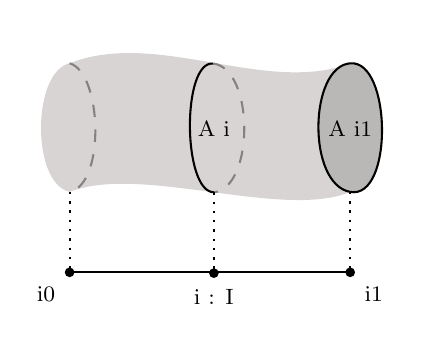
\begin{tikzpicture}[x=0.75pt,y=0.75pt,yscale=-1,xscale=1,roundnode/.style={circle, fill=black, inner sep=0pt, minimum size=3.5pt}]
  %uncomment if require: \path (0,300); %set diagram left start at 0, and has height of 300
  
  %Straight Lines [id:da9992281795763605] 
  \draw    (38.49,139.28) -- (173.68,139.28) ;
  \node[roundnode, label=south west:{\footnotesize{\con{i0}}}] (I0) at (38.49,139.28) {} ;
  \node[roundnode, label=south east:{\footnotesize{\con{i1}}}] (I0) at (173.68,139.28) {} ;
  %Straight Lines [id:da39034223732541395] 
  \draw  [dash pattern={on 0.84pt off 2.51pt}]  (38.49,100.54) -- (38.49,139.28) ;
  %Straight Lines [id:da7047440344843311] 
  \draw  [dash pattern={on 0.84pt off 2.51pt}]  (173.68,100.54) -- (173.68,139.28) ;
  %Shape: Polygon Curved [id:ds1909563977441432] 
  \draw  [draw opacity=0][fill={rgb, 255:red, 216; green, 212; blue, 212 }  ,fill opacity=1 ] (38.49,38.57) .. controls (80.7,21.91) and (132.97,54.06) .. (173.68,38.57) .. controls (155.5,42.83) and (154.6,97.83) .. (173.68,100.54) .. controls (157.68,107.2) and (133.03,104.05) .. (108.05,100.73) .. controls (82.13,97.28) and (55.85,93.64) .. (38.49,100.54) .. controls (19.86,96.28) and (20.31,42.83) .. (38.49,38.57) -- cycle ;
  %Shape: Polygon Curved [id:ds8315502681665057] 
  \draw  [fill={rgb, 255:red, 186; green, 183; blue, 183 }  ,fill opacity=1 ] (173.68,100.54) .. controls (194.56,104.29) and (193.65,36.89) .. (173.68,38.57) .. controls (153.7,40.24) and (152.8,96.8) .. (173.68,100.54) -- cycle ;
  %Curve Lines [id:da7321879710524096] 
  \draw [color={rgb, 255:red, 130; green, 130; blue, 130 }  ,draw opacity=1 ] [dash pattern={on 4.5pt off 4.5pt}]  (38.49,38.57) .. controls (54.11,42.96) and (55.91,96.8) .. (38.49,100.54) ;
  %Curve Lines [id:da30123038239331235] 
  \draw    (108.05,100.73) .. controls (92.86,100.67) and (92.41,37.14) .. (107.73,38.69) ;
  %Curve Lines [id:da051040178779523826] 
  \draw [color={rgb, 255:red, 130; green, 130; blue, 130 }  ,draw opacity=1 ] [dash pattern={on 4.5pt off 4.5pt}]  (107.73,38.69) .. controls (127.56,41.41) and (127.56,98.35) .. (108.05,100.73) ;
  %Straight Lines [id:da44514618287884566] 
  \draw  [dash pattern={on 0.84pt off 2.51pt}]  (108,100.73) -- (108,139.67) ;
  \node (AI) at (108,70) {\footnotesize{\var{A}~\var{i}}} ;
  \node (AI1) at (173.7,70) {\footnotesize{\var{A}~\con{i1}}} ;
  \node[roundnode, label=south:{\footnotesize{\var{i} : \func{I}}}] (SI) at (108,139.67) {} ;
  
  \end{tikzpicture}
  \caption{Graphical representation of a line of types 
    \( A : \func{I} \to \func{Set}\ \var{ℓ} \), or equivalently a type depending 
    on \( i : \func{I} \)}
\end{figure}

Given a line of types \( A : \func{I} \to \func{Set}\ \var{ℓ} \), we can form 
the type of \emph{dependent lines} \( (i : \func{I}) \to A\ i \).
And since it is often useful to specify the endpoints of a line, 
\CubicalAgda provides primitive
\sideremark{we omit the quantification of the universe level \var{ℓ} for readability}
\emph{path types} that add constraints on the endpoints:
%
\ExecuteMetaData[chapters/literate-agda/Code.tex]{PathP}

Paths are introduced by lambda abstractions:
\begin{mathpar}
  \inferrule{\Gamma,\; i : \func{I}\enskip \vdash \enskip t : A\ i}
  {\Gamma \enskip \vdash \enskip \symb{λ} \var{i} \to t : \func{PathP}\;\var{A}\;t[\substnop {i}
  {\con{i0}}]\;t[\substnop {i} {\con{i1}}]}
\end{mathpar}
Then given $\var{p} : \func{PathP}\;\var{A}\;\var{a}_0\;\var{a}_1$, we can apply
it to $\var{r} : \func{I}$ and obtain
$\var{p}\;\var{r} : \var{A}\;\var{r}$. 
% 
And we always have that
$\var{p}\;\con{i0}$ is convertible to $a_0$ and $\var{p}\;\con{i1}$ is
convertible to $a_1$, even when \( p \) is a neutral term.

The type \func{PathP} plays the role of propositional equality in cubical type theory.
More specifically it has the role of heterogeneous equality, since the two 
endpoints are in different types; this is similar to the dependent paths in
HoTT~\sidecite[][Sect. 6.2]{hottbook}. We define the type of homogeneous
paths/equalities in terms of \func{PathP} as follows:
% 
\sideremark{The homogeneous path types are written using a triple equality
  symbol, following the convention of \CubicalAgda. This has nothing
  to do with the definitional equality of \cref{ch:observational} or the 
  reducible equality of \cref{ch:metatheory}.}
% 
\ExecuteMetaData[chapters/literate-agda/Code.tex]{Path} %

The syntax $\{\var{A} = A\}$ in the definition tells \Agda to bind the hidden
argument \var{A} (first occurence) to a variable $A$ (second occurence) that 
can be used on the right hand side of the definition. 
Viewing equalities as paths allows us to reason about equality; for
instance the constant path represents a proof of equality by reflexivity.
%
\ExecuteMetaData[chapters/literate-agda/Code.tex]{refl}

% We can also directly apply a function to a path in order to prove that
% dependent functions respect path equality, as shown in the definition
% of \func{cong} below.  Simply by computation \func{cong} satisfies
% some new definitional equalities compared to the corresponding
% definition for the inductive equality type à la \sidecitet{MartinLoef75}.
% For instance, \func{cong} is functorial by definition: we can prove
% \func{congId} and \func{congComp} by plain reflexivity (\func{refl}).
% %
% \ExecuteMetaData[chapters/literate-agda/Code.tex]{cong}

Using path types as equalities lets us prove theorems that are not provable in
standard \Agda. For example, the principle of function extensionality (which states
that two pointwise equal functions are equal) has a very simple proof:
% 
\ExecuteMetaData[chapters/literate-agda/Code.tex]{funext}
% 
\sideremark[*-4]{When we input this definition to \CubicalAgda, 
  the proof assistant checks that \( p\ x\ i \) is convertible to \( f\ x \)
  when \( i = \con{i0} \) and convertible to \( g\ x \) when \( i = \con{i1} \).
  And it is indeed the case, because \( p\ x \) has type \( f\ x\ \func{≡}\ g\ x \).}

The proof of function extensionality for dependent and $n$-ary
functions is equally easy. Since $\func{funExt}$ is a
theorem and not an axiom, it has computational
content: it simply swaps the arguments to \var{p}.

We can also use the de Morgan structure on \func{I} to construct various
useful operations, for example the \emph{reversal} of a path is defined
using \func{∼{}\_} and encodes the fact that \func{≡} is symmetric.
%
\sideremark{In this definition, the boundary conditions are met because
  \( \text{\func{∼{}}} \con{i0} = \con{i1} \) and 
  \( \text{\func{∼{}}} \con{i1} = \con{i0} \)}
% 
\ExecuteMetaData[chapters/literate-agda/Code.tex]{sym}

\subsection{Transport and Composition}

\paragraph*{Transport}
% 
One of the basic uses of the propositional equality in type theory is 
to perform \emph{type coercions}: 
% 
given an equality/path between two types \( A \) and \( B \), we should get
a function from \( A \) to \( B \).
% 
In \CubicalAgda this is the job of the \func{transport} operator,
which is defined in terms of the more general operator \func{transp}.
%
\ExecuteMetaData[chapters/literate-agda/Code.tex]{transport}
% 
The \func{transp} operator is a primitive object in cubical type theory,
and it satisfies complex computation rules.
% 
But \func{transport} will be sufficient for the purposes of this chapter.

Using transport, we can substitute a term with another path-equal term.
%
\sideremark{This function invokes \func{transport} with a proof that the family
$B$ respects the equality $p$:
\[
  \lambda\;i \to B\;(p\;i) : B\;x\;\func{≡}\;B\;y
\]}
% 
\ExecuteMetaData[chapters/literate-agda/Code.tex]{subst}

If we combine the transport operator with some simple de Morgan algebra, we 
can even define an induction principle for paths that resembles 
the \( J \) eliminator for Martin-Löf's inductively defined identity 
types~\sidecite{MartinLoef75}.
%
\ExecuteMetaData[chapters/literate-agda/Code.tex]{J}

However, an important difference between the cubical path types and
Martin-Löf's identity types (and the path types in axiomatic HoTT) is that
cubical path types are not inductive types.
% 
And in particular, the above definition does not satisfy the computation 
rule when applied to \func{refl}. 
% 
Nevertheless, we can still prove that it holds up to a path:
% 
\sideremark{In this sense, the cubical equality is similar to the observational
  equality of \cref{ch:observational}: both provide new extensionality principles 
  in exchange for a weakening the computation rule of \( J \) to a propositional 
  equality.}
%
\ExecuteMetaData[chapters/literate-agda/Code.tex]{Jrefl}

Readers who are familiar with HoTT might be worrying that this weakened
computation rule may complicate proofs; however in our experience this 
is rarely the case, because most proofs done \textit{via} path induction 
in HoTT can be done in more direct ways using cubical primitives.
% 
% Furthermore, for closed terms (potentially depending on interval variables) 
% the lack of this definitional equality in cubical type theory does not affect 
% canonicity, in particular any closed term of type natural numbers is 
% definitionally equal to a numeral as proved by~\sidecitet{Huber16}

\paragraph*{Composition}
% 
Cubical type theory also provides a primitive operation called \emph{homogeneous 
composition} which allows us to compose paths and more generally, to compose 
higher dimensional cubes. 

In order to describe homogeneous composition, we need to have a notion of 
partially specified $n$-dimensional cubes, \ie cubes where some faces are 
missing. 
% 
For this reason, cubical type theory allows us to manipulate \emph{partial terms}:
in \CubicalAgda, the type \func{Partial}~\var{r}~\var{A} contains elements of
% 
\sideremark{In the type \func{Partial}~\var{r}~\var{A}, the second argument \( r \)
  is an element of \func{I} that is used to select faces from the context. 
  For instance if the context contains two variables \( i, j \) of type \func{I}, 
  then every term we define naturally has the shape of a square. Then the constraint
  \( {i~\func{∨}~j = \con{i1}} \) selects a union of two faces of the square.}
% 
\var{A} which are only defined when (\var{r} = \con{i1}) holds. 
% 
For instance, if we are working in context that contains a variable \( i : \func{I} \) 
and \( A \) is a well-formed type, we can 
form the type \func{Partial}~(\var{i}~\func{∨}~\func{∼{}}~\var{i})~\var{A} 
of elements of \( A \) which are defined when \( \var{i} = \con{i1} \)
or when \( \var{i} = \con{i0} \).

In \CubicalAgda, elements of partial cubical types are introduced with 
pattern-matching on the constraint.
% 
For this purpose \CubicalAgda adds support for a new type of patterns, 
of which $(\var{i} = \con{i1})$ and $(\var{i} = \con{i0})$ are examples in
the following definition.
%
\ExecuteMetaData[chapters/literate-agda/Code.tex]{partialBoolTwo}

To help differentiate them from normal pattern matching on inductive types,
we will write partial elements with pattern-matching lambdas.
% 
\ExecuteMetaData[chapters/literate-agda/Code.tex]{partialBool'}

The term \func{partialBool} should be thought of as a boolean
depending on \var{i} with different values when \var{i} is \con{i1}
and when \var{i} is \con{i0}.
This is only defined on the two endpoints of \func{I} and there is no
way to extend this partial type to a regular dependent boolean, or otherwise
we would get a path between \con{true} and \con{false}.\\

\begin{figure}[!h]
\tikzset{every picture/.style={line width=0.75pt}} %set default line width to 0.75pt        

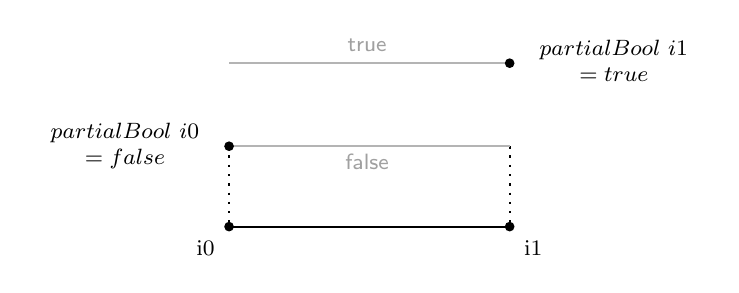
\begin{tikzpicture}[x=0.75pt,y=0.75pt,yscale=-1,xscale=1,roundnode/.style={circle, fill=black, inner sep=0pt, minimum size=3.5pt}]
  %uncomment if require: \path (0,300); %set diagram left start at 0, and has height of 300

%Straight Lines [id:da9992281795763605] 
\draw    (38.49,139.28) -- (173.68,139.28) ;
\node[roundnode, label=south west:{\footnotesize{\con{i0}}}] (I0) at (38.49,139.28) {} ;
\node[roundnode, label=south east:{\footnotesize{\con{i1}}}] (I0) at (173.68,139.28) {} ;
%Straight Lines [id:da39034223732541395] 
\draw  [dash pattern={on 0.84pt off 2.51pt}]  (38.49,100.54) -- (38.49,139.28) ;
%Straight Lines [id:da7047440344843311] 
\draw  [dash pattern={on 0.84pt off 2.51pt}]  (173.68,100.54) -- (173.68,139.28) ;
%Straight Lines [id:da4797898542184591] 
\draw [color={rgb, 255:red, 180; green, 180; blue, 180 }  ,draw opacity=1 ]   (38.49,100.54) -- (173.68,100.54) ;
%Straight Lines [id:da557351613724285] 
\draw [color={rgb, 255:red, 180; green, 180; blue, 180 }  ,draw opacity=1 ]   (38.49,60.54) -- (173.68,60.54) ;
\node[roundnode, label=east:{\footnotesize{\( \begin{array}{c} \AgdaFunction{partialBool}\ \con{i1} \\ = \con{true} \end{array} \)}}] (TT) at (173.68,60.54) {} ;
\node[roundnode, label=west:{\footnotesize{\( \begin{array}{c} \AgdaFunction{partialBool}\ \con{i0} \\ = \con{false} \end{array} \)}}] (FF) at (38.49,100.54) {} ;
\node (TR) at (105,52) {\textcolor[RGB]{160,160,160}{\footnotesize\textsf{true}}} ;
\node (TR) at (105,108) {\textcolor[RGB]{160,160,160}{\footnotesize\textsf{false}}} ;

\end{tikzpicture}
\caption{Graphical representation of the partial element \func{partialBool}}
\end{figure}

Cubical type theory also provides \emph{cubical subtypes}~\sidecite{CCHM}.
Given a type \( {\var{A} : \func{Set}~\var{ℓ}} \), a face constraint encoded
by an element of the interval \( {\var{r} : \func{I}} \) and a partial term 
\( {\var{u}~:~\func{Partial}~\var{r}~\var{A}} \), we can form the type
\( {\var{A}~\func{[}~\var{r}~\func{↦}~\var{u}~\func{]}} \)
of total elements of \( A \) that extend \( u \).  
% 
A term \var{v} of this type is a term of type \var{A} that is definitionally equal to
\var{u} when the constraint (\var{r} = \con{i1}) holds. 

Any term \var{u} : \var{A} can be seen as a term of type
\var{A}~\func{[}~\var{r}~\func{↦}~\var{u}~\func{]} that agrees with
itself when (\var{r} = \con{i1}) holds.
%
\ExecuteMetaData[chapters/literate-agda/Code.tex]{inc}

We can also forget that a partial element agrees with \var{u} when
\var{r} = \con{i1}.
%
\ExecuteMetaData[chapters/literate-agda/Code.tex]{ouc}

And these two operations are inverse to each other when well-typed. Using
this cubical infrastructure we can now give the type of the
homogeneous composition operation.
% that generalizes binary composition of paths so that we can compose
% multiple composable cubes.
%
\ExecuteMetaData[chapters/literate-agda/Code.tex]{hcomp}

The meaning of this type is a bit opaque in first approach.
% 
To get a clearer picture of \func{hcomp}, we can start by looking at the special
case
\func{hcomp}~\{\var{r}~=~\var{i}~\func{∨}~\func{∼{}}~\var{i}\}~\var{u}~\var{t},
where assume that we are working in a context that contains the interval 
variable \( i \)---in other words, \( A \) is a type indexed over the interval 
\func{I} as pictured in \cref{fig:hcomp-demo}.
 
Then \var{t} is a total element of \( A \) and \var{u} extends \( t \)
when \( i = \con{i0} \) or \( i = \con{i1} \), resulting in the shape of
an open box.
% 
\CubicalAgda makes sure that \var{t} agrees with \var{u}~\con{i0} when the
constraint is satisfied; this is specified by making \var{t} an extension type. 
% 
The \func{hcomp} operation then gives us the missing side of the box.

\begin{figure}[!h]
  \tikzset{every picture/.style={line width=0.75pt}} %set default line width to 0.75pt        

  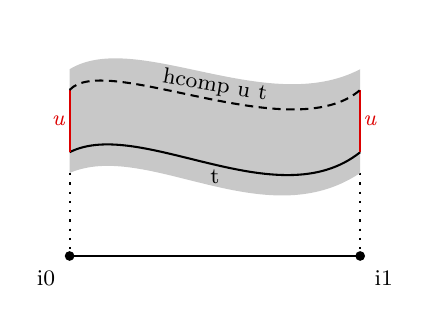
\begin{tikzpicture}[x=0.75pt,y=0.75pt,yscale=-1,xscale=1,roundnode/.style={circle, fill=black, inner sep=0pt, minimum size=3.5pt}]
  %uncomment if require: \path (0,300); %set diagram left start at 0, and has height of 300
  \node[roundnode, label=south west:{\footnotesize{\con{i0}}}] (I0) at (40,140) {} ;
  \node[roundnode, label=south east:{\footnotesize{\con{i1}}}] (I0) at (180,140) {} ;
  %Straight Lines [id:da9992281795763605] 
  \draw    (40,140) -- (180,140) ;
  %Straight Lines [id:da39034223732541395] 
  \draw  [dash pattern={on 0.84pt off 2.51pt}]  (40,100) -- (40,140) ;
  %Straight Lines [id:da7047440344843311] 
  \draw  [dash pattern={on 0.84pt off 2.51pt}]  (180,100) -- (180,140) ;
  %Shape: Polygon Curved [id:ds6871817755174879] 
  \draw  [draw opacity=0][fill={rgb, 255:red, 200; green, 200; blue, 200 }  ,fill opacity=1 ] (40,50) .. controls (72.17,30.5) and (135.17,73.5) .. (180,50) .. controls (179.92,99.92) and (179.92,50.17) .. (180,100) .. controls (133.67,131) and (77.17,84) .. (40,100) .. controls (39.92,50.17) and (39.92,99.92) .. (40,50) -- cycle ;
  %Curve Lines [id:da27064595952926185] 
  \draw    (40,90) .. controls (74,72.83) and (140,121.83) .. (180,90) ;
  %Straight Lines [id:da9072242715265223] 
  \draw  [color={rgb, 255:red, 220; green, 0; blue, 0 }  ,draw opacity=1 ]  (40,90) -- (40,60) ;
  %Straight Lines [id:da34146717098575696] 
  \draw  [color={rgb, 255:red, 220; green, 0; blue, 0 }  ,draw opacity=1 ]  (180,60) -- (180,90) ;
  %Curve Lines [id:da40884349871839487] 
  \draw  [dash pattern={on 3pt off 2pt}]  (40,60) .. controls (57.25,41.25) and (146.83,88.5) .. (180,60) ;
  
  \node (T) at (110,102) {\footnotesize\var{t}} ;
  \node (U1) at (35,75) {\textcolor[RGB]{220,0,0}{\footnotesize\textit{u}}} ;
  \node (U2) at (185,75) {\textcolor[RGB]{220,0,0}{\footnotesize\textit{u}}} ;
  \node[rotate=-10] (H) at (110,58) {\footnotesize{\func{hcomp}~\var{u}~\var{t}}} ;

  \end{tikzpicture}
  \caption{Graphical representation of the homogeneous composition \func{hcomp}~\{\var{r}~=~\var{i}~\func{∨}~\func{∼{}}~\var{i}\}~\var{u}~\var{t}}
  \label{fig:hcomp-demo}
\end{figure}

The general case does pretty much the same, but with an arbitrary number of
dimension and an arbitrary face constraint.
As an example for the use of \func{hcomp}, we can define binary composition of paths:
%
\ExecuteMetaData[chapters/literate-agda/Code.tex]{compPath}

Pictorially we are given \var{p} : \var{x} \ \func{≡}\  \var{y} and
\var{q} : \var{y} \ \func{≡}\  \var{z}, and the composite of the two paths
is obtained by computing the dashed top of the following square.
%
\begin{figure}[!h]
\begin{mathpar}
  \vcenter{\hbox{\begin{tikzpicture}[baseline=40,->, scale=0.8]
    \node [anchor=west] (x) at (0, 1) {\footnotesize \( j \)};
    \node [anchor=north] (y) at (1, 0) {\footnotesize \( i \)};
    \draw (0,0) -- (0,1);
    \draw (0,0) -- (1,0);
  \end{tikzpicture}}}
  \and %
  \qquad
    \begin{tikzpicture}[baseline=30,xscale=2,yscale=2]
    \node (A01) at (0,1) {\var{x}};
    \node (A11) at (1,1) {\var{z}};
    \node (A00) at (0,0) {\var{x}};
    \node (A10) at (1,0) {\var{y}};
    \path[->,font=\scriptsize,>=angle 90]
      (A00) edge node[left]{\var{x}} (A01)
      (A10) edge node[right]{\var{q} \var{j}} (A11)
      (A00) edge node[below]{\func{inS} (\var{p} \var{i})} (A10);
    \path[->,font=\scriptsize,>=angle 90,dashed]
      (A01) edge node[above]{} (A11);
  \end{tikzpicture}

\end{mathpar}
\caption{Composing two paths using \func{hcomp}}
\end{figure}

% As we are constructing a path from \var{x} to \var{z} along \var{i}
% we have \var{i} : \func{I} in context and put \func{inS} (\var{p}
% \var{i}) as bottom. The direction \var{j} is abstracted in the first
% argument to \func{hcomp} and we use pattern matching to specify the
% sides.

% We can also define homogeneous filling of open boxes as
% %
% \ExecuteMetaData[chapters/literate-agda/Code.tex]{hfill}
% % \andreas{Starting here, I cannot comprehend the definitions any more.
% % There are now three dimensions involved: $r$, $i$, $j$, and I do not
% % know how to map this to the picture.}

% When \var{i} is \con{i0} this is \func{outS}~\var{t} and when \var{i}
% is \con{i1} it is \func{hcomp} ($\lambda$ \var{j} $\to$ $\lambda$ \{
% (\var{r} = \con{i1}) $\to$ \var{u} \var{j} \func{1=1} \} \var{t} as
% the absurd faces (\con{i0} = \con{i1}) gets filtered out. By the extensionality of
% partial elements this hence gives a line along \var{i}
% between \func{outS}~\var{t} and \func{hcomp} \var{u} \var{t} which
% geometrically corresponds to the filling of an open box as it connects
% the base with the lid computed using \func{hcomp}. %
% %% \anders{Is this clearer now?} %
% %% \andreas{It is plausible that there is a beta rule $\func{outS} \circ
% %%   \func{inS}
% %%   = \func{id}$, however, it should be mentioned in the
% %%   subsection before.  Is there also an eta rule?  Otherwise, how do you
% %%   reason? And if there is eta, under which condition does it hold?
% %%   Should be added to the previous subsection.} %
% In the special case when \var{q} is \func{refl} the filler of the
% above square gives us a direct cubical proof that composing \var{p}
% with \func{refl} is \var{p}.
% %
% \ExecuteMetaData[chapters/literate-agda/Code.tex]{compPathRefl}

By composing paths and higher cubes using \func{hcomp}, we can reason
about equalities/paths in a very direct way, avoiding the use of path
induction.

\subsection{Higher Inductive Types}
\label{sec:hits}

\CubicalAgda has native support for HITs, which means that we
can define the circle using an \Agda~\keyw{data} declaration.
\ExecuteMetaData[chapters/literate-agda/Circle.tex]{s1}

% \begin{minipage}{0.4\linewidth}
% \ExecuteMetaData[chapters/literate-agda/Torus.tex]{s1}
% \end{minipage}
% \begin{minipage}{0.6\linewidth}
% \begin{center}
% \begin{tikzpicture}
%   \draw[->,thick,draw=black,solid,line width=0.3mm]
%   (0:0) node[above]{\con{base}} arc[radius=0.6, start angle=90, end
%   angle=-265];
%   \node[] at (0,0) (b) {$\bullet$};
%   \node[] at (1,-0.58) (b) {\con{loop}};
% \end{tikzpicture}
% \\\ \\
% \end{center}
% \end{minipage}

This is a type with a point constructor \con{base} and a nontrivial
equality / path constructor \con{loop} connecting \con{base} to itself
as shown in the drawing below.

\begin{figure}[!h]
\begin{center}
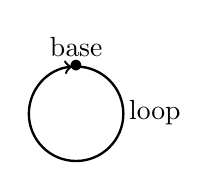
\begin{tikzpicture}
  \draw[->,thick,draw=black,solid,line width=0.3mm]
  (0:0) node[above]{\con{base}} arc[radius=0.6, start angle=90, end
  angle=-265];
  \node[] at (0,0) (b) {$\bullet$};
  \node[] at (1,-0.58) (b) {\con{loop}};
\end{tikzpicture}
\end{center}
\caption{Graphical representation of the HIT \func{S¹}}
\end{figure}

Functions out of HITs are written using normal \Agda pattern
matching equations. The following function wraps the circle twice
around itself, by composing the \con{loop} constructor with itself:
%
\sideremark{When we input this definition by pattern matching, \CubicalAgda 
  checks that the boundary constraints from the definition of \func{S¹} are
  respected: since \con{loop}~\con{i0}~=~\con{base} and 
  \con{loop}~\con{i1}~=~\con{base}, we want to have 
  \func{double}~(\con{loop}~\con{i0})~=~\func{double}~\con{base} 
  and \func{double}~(\con{loop}~\con{i1})~=~\func{double}~\con{base}.}
% 
\ExecuteMetaData[chapters/literate-agda/Circle.tex]{double}

Both cases define a \emph{definitional} equality, while in axiomatic HoTT
this would have had to be defined using the postulated recursion
principle for the circle. This means that in HoTT \func{double}
applied to \con{loop} would not reduce automatically, but a
proof of equality would instead have to be applied
manually. This leads to rather bureaucratic proofs as one then has to
handle these explicit applications of the computation rule when
reasoning about \func{double}. Furthermore, this is not very natural
if one wants to use HITs for programming.

In order for the circle to be the free type generated by \con{base}
and \con{loop}, it also needs to have elements of the form \con{loop}
$\cdot$ \con{loop} as in the above definition of \func{double}. 
% 
In general, for HITs 
$\func{hcomp}\;(\lambda\,i\to\lambda~\{~(r = \io) \to u\})\;u_0$ 
only reduces to u[\substnop i {\io}] when $r$ is $\io$, and is
considered to be a canonical element otherwise. The circle hence has
constructors of the form $\hcompcon~u~u_0$ in addition to \con{base}
and \con{loop}. 

% \[
%   \func{double}~(\con{loop}~\iz) = \func{double}~\con{base} = \con{base}
% \]
% is the same as
% \[
%   \func{double}~(\con{loop}~\iz) = (\con{loop} \cdot \con{loop})~\iz = (\hcompcon~...~...)~\iz = \con{base}
% \]
% and similarly when \var{i} is \io.
% \loic{I think this could be more clear, we should spell out that these are
%   two different ways to rewrite the same term or something.}
% \anders{I agree. Maybe we don't even have to say it in this much detail.}

\subsection{Glue Types and Univalence}

The final ingredient of cubical type theory relevant for this chapter
are the \func{Glue} types of \sidecitet{CCHM} that let us give
computational content to univalence. Given that a type in cubical type
naturally has the shape of a higher dimensional cube, \func{Glue} types let us
replace the faces of these cubes with some \emph{equivalent} types.
% This is analogous to how \func{hcomp} lets us replace some
% faces of a cube by composing it with other cubes, however for
% \func{Glue} types we can compose with equivalences instead of paths.
% \anders{Ok, if you have some better way of explaining Glue informally
%   please do so! Maybe we don't really have to talk about Glue in any
%   detail though if the only thing we use is ua...}  \loic{I was only
%   saying this for the \func{hcomp} analogy which is less clear, this
%   is a good description of glue imo. And we do need it for Hopf.}

There are many ways to define the notion of ``equivalence of types''
in HoTT; \CubicalAgda uses the definition that two types are
equivalent if there is a function between them with
\emph{``contractible fibers''} following the terminology of
\sidecitet{Voevodsky15} and the HoTT book~\sidecite{HottBook13}. Spelled out,
a map $f : A \to B$ is an equivalence if the preimage of any point in
\var{B} is a singleton type. 
% 
\sideremark{Equivalences are formally defined as follows:\\
\func{isEquiv}~f\ =\ (\var{y}~:~\var{B})~\to~\func{isContr}~(\func{fiber}~\var{f}~\var{y})\\
\func{fiber}~\var{f}~\var{y}\ =\ \func{Σ}~(\var{x}~:~\var{A})~.~\var{f}~\var{x}~\func{≡}~\var{y} \\
\func{isContr}~\var{A}\ =\ \func{Σ}~(\var{a}~:~\var{A})~.~((\var{x}~:~\var{A})~\to~\var{x}~\func{≡}~\var{a})}
% 
We write \var{A} \func{≃} \var{B} if
there is a chosen equivalence $f : A \to B$ between \var{A} and
\var{B}. A key result is that isomorphisms, in the sense of a
section-retraction pair of functions, give rise to equivalences.
In particular, the identity function is an equivalence:
$\func{idEquiv}~\var{A}~:~\var{A}~\func{≃}~\var{A}$.

\ExecuteMetaData[chapters/literate-agda/Glue.tex]{Glue}

The \func{Glue} primitive takes a base type \var{B}, a constraint \var{r} and 
a partial family of types \var{A} that are equivalent to \var{B} when 
\var{r}~=~\con{i1} holds, and produces type by ``gluing'' \var{A} onto \var{B}.
% 
The resulting type is definitionally equal to \var{A} when the constraint 
\var{r}~=~\con{i1} holds.

\begin{figure}[!h]
  \tikzset{every picture/.style={line width=0.75pt}} %set default line width to 0.75pt        

  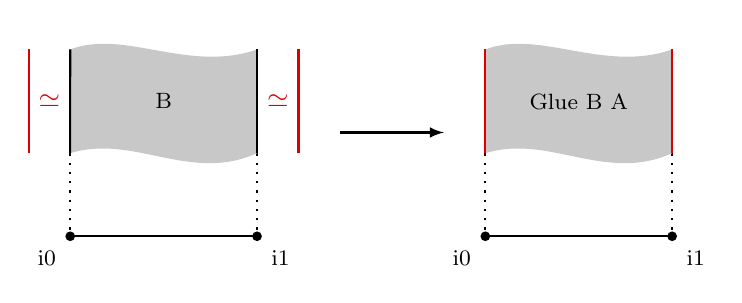
\begin{tikzpicture}[x=0.75pt,y=0.75pt,yscale=-1,xscale=1,roundnode/.style={circle, fill=black, inner sep=0pt, minimum size=3.5pt}]
  %uncomment if require: \path (0,300); %set diagram left start at 0, and has height of 300
  \node[roundnode, label=south west:{\footnotesize{\con{i0}}}] (I0) at (40,140) {} ;
  \node[roundnode, label=south east:{\footnotesize{\con{i1}}}] (I0) at (130,140) {} ;
  \node[roundnode, label=south west:{\footnotesize{\con{i0}}}] (I0) at (240,140) {} ;
  \node[roundnode, label=south east:{\footnotesize{\con{i1}}}] (I0) at (330,140) {} ;
  
  %Straight Lines [id:da9992281795763605] 
  \draw    (39.98,140) -- (130,140) ;
  %Straight Lines [id:da39034223732541395] 
  \draw  [dash pattern={on 0.84pt off 2.51pt}]  (39.98,100) -- (39.98,140) ;
  %Straight Lines [id:da7047440344843311] 
  \draw  [dash pattern={on 0.84pt off 2.51pt}]  (130,100) -- (130,140) ;
  %Shape: Polygon Curved [id:ds6871817755174879] 
  \draw  [draw opacity=0][fill={rgb, 255:red, 200; green, 200; blue, 200 }  ,fill opacity=1 ] (39.98,50) .. controls (66,40) and (97,61.5) .. (130,50) .. controls (129.95,99.92) and (129.95,50.17) .. (130,100) .. controls (97.5,114.5) and (70.5,90.5) .. (39.98,100) .. controls (39.92,50.17) and (39.92,99.92) .. (39.98,50) -- cycle ;
  %Straight Lines [id:da9551336451182719] 
  \draw [color={rgb, 255:red, 220; green, 0; blue, 0 }  ,draw opacity=1 ]   (150,50) -- (150,100) ;
  %Straight Lines [id:da23306158989109416] 
  \draw [color={rgb, 255:red, 220; green, 0; blue, 0 }  ,draw opacity=1 ]   (20,50) -- (20,100) ;
  %Straight Lines [id:da2010301085745465] 
  \draw    (239.98,140) -- (330,140) ;
  %Straight Lines [id:da3537038075493171] 
  \draw  [dash pattern={on 0.84pt off 2.51pt}]  (239.98,100) -- (239.98,140) ;
  %Straight Lines [id:da9379434659446393] 
  \draw  [dash pattern={on 0.84pt off 2.51pt}]  (330,100) -- (330,140) ;
  %Shape: Polygon Curved [id:ds001846376488208623] 
  \draw  [draw opacity=0][fill={rgb, 255:red, 200; green, 200; blue, 200 }  ,fill opacity=1 ] (239.98,50) .. controls (266,40) and (297,61.5) .. (330,50) .. controls (329.95,99.92) and (329.95,50.17) .. (330,100) .. controls (297.5,114.5) and (270.5,90.5) .. (239.98,100) .. controls (239.92,50.17) and (239.92,99.92) .. (239.98,50) -- cycle ;
  %Straight Lines [id:da011720172503938642] 
  \draw [color={rgb, 255:red, 220; green, 0; blue, 0 }  ,draw opacity=1 ]   (330,50) -- (330,100) ;
  %Straight Lines [id:da4784036579630343] 
  \draw [color={rgb, 255:red, 220; green, 0; blue, 0 }  ,draw opacity=1 ]   (239.98,50) -- (239.98,100) ;
  %Straight Lines [id:da289164093987879] 
  \draw    (130,50) -- (130,100) ;
  %Straight Lines [id:da8905847731459658] 
  \draw    (40,50) -- (39.98,100) ;
  %Straight Lines [id:da9372757307556213] 
  \draw[-latex]   (170,90) -- (220,90) ;
  
  \node (E1) at (140, 75) {\textcolor[RGB]{220,0,0}{\( \simeq \)}} ;
  \node (E2) at (30, 75) {\textcolor[RGB]{220,0,0}{\( \simeq \)}} ;
  \node (B) at (85, 75) {\footnotesize{\var{B}}} ;
  \node (GB) at (285, 75) {\footnotesize{\func{Glue}~\var{B}~\var{A}}} ;
  \end{tikzpicture}
  \caption{Graphical representation of 
    \func{Glue}~\var{B}~\{\var{r}~=~\var{i}~\func{∨}~\func{∼{}}~\var{i}\}~\var{A}.
    We start with a type \var{B} indexed over \func{I} and we replaced its faces
    with equivalent types.}
\end{figure}
Elements of a \func{Glue} type are introduced using the \func{glue} constructor 
and eliminated using the \func{unglue} operation. 
% 
Examples of this will be discussed in the proof of \cref{thm:hopf}. 

With \func{Glue} types, we can turn an equivalence of types into a path:
%
\ExecuteMetaData[chapters/literate-agda/Glue.tex]{ua}

The idea is that we glue \var{A} onto \var{B} when \var{i} is \con{i0}
using \var{e} and \var{B} onto itself when \var{i} is \con{i1} using
the identity equivalence. The term \func{ua} \var{e} is a path from
\var{A} to \var{B} as the \func{Glue} type reduces when the face
conditions are satisfied---when \var{i} is \con{i0} this reduces to
\var{A} and when \var{i} is \con{i1} it reduces to \var{B}. %

The univalence axiom is a little more complex, since it asks for the obvious 
function \var{A}~\func{≡}~\var{B}~\to~\var{A}~\func{≃}~\var{B} to be an 
equivalence.
% 
We can also derive it from \func{Glue}, but for all of the examples in this 
chapter the \func{ua} function will be sufficient.

% A consequence is that whenever we have an equivalence
% $e : A\;\func{≃}\;B$ we have that
% $\func{transport}\;(\symb{λ}\;i\;\func{→}\;F\;(\func{ua}\;e\;i))$ is
% an equivalence as well. This ability to lift equivalences through
% arbitrary type operators $F$ is an easily overlooked benefit of a
% language with computational univalence.

\section{The Circle and Torus}
\label{sec:torus}

We already gave the definition of the circle as a HIT in \cref{sec:hits}. 
Similarly, we can define the torus as a datatype in \CubicalAgda as follows:
%
\ExecuteMetaData[chapters/literate-agda/Torus.tex]{torus}

The idea is that the \func{Torus} has a base \con{point} with two
nontrivial path constructors connecting it to itself and a
\con{square} relating the two paths. This square can be illustrated
by:
%
\begin{figure}[!h]
\begin{tikzpicture}[xscale=2,yscale=2]
  \draw [thin,->] (-1.55,0) -- (-1.55,0.4) ;
  \draw [thin,->] (-1.55,0) -- (-1.15,0) ;
  \node [anchor=north] (x) at (-1.15, 0) {\footnotesize \( i \)};
  \node [anchor=west] (y) at (-1.55, 0.4) {\footnotesize \( j \)};

  \node (A01) at (0,1) {\con{point}};
  \node (A11) at (1,1) {\con{point}};
  \node (A00) at (0,0) {\con{point}};
  \node (A10) at (1,0) {\con{point}};
  \node (C) at (0.5,0.5) {\con{square}};
  \path[->,>=angle 90]
    (A01) edge node[above]{\con{line1}} (A11)
    (A00) edge node[left]{\con{line2}} (A01)
    (A10) edge node[right]{\con{line2}} (A11)
    (A00) edge node[below]{\con{line1}} (A10);
\end{tikzpicture}
\caption{The two-dimensional face of the torus}
\end{figure}

The type of the \con{square} constructor captures this by identifying
\con{line2} with itself \emph{over} \con{line1}.  In order to see that
this represents a torus imagine \con{square} being made of a piece of
paper that is folded so that the opposite sides are matched up.  The
proof that the \func{Torus} type is equivalent to two circles in
\CubicalAgda was given by \sidecitet[][Section 2.4.1]{cubicalagda},
but we recall it here for completeness. We first write a function from
the torus to two circles using pattern matching.
%
\ExecuteMetaData[chapters/literate-agda/Torus.tex]{t2c}
% \noindent\begin{minipage}[t]{0.55\linewidth}
%   \ExecuteMetaData[chapters/literate-agda/Torus.tex]{t2c}
% \end{minipage}
% \begin{minipage}[t]{0.5\linewidth}
%   \ExecuteMetaData[chapters/literate-agda/Torus.tex]{c2t}
% \end{minipage}

To prove that this is an equivalence we need to define its inverse
\func{c2t}~:~\func{S¹}~\func{×}~\func{S¹}~→~\func{Torus}. This
function is also defined by pattern matching in the obvious
way. Proving that the two maps cancel is then simply done by
pattern matching with \func{refl} in all cases.
%
\ExecuteMetaData[chapters/literate-agda/Torus.tex]{c2tt2c}
% \begin{center}
% \begin{minipage}[t]{1.0\linewidth}
% \begin{minipage}[t]{0.5\linewidth}
%   \ExecuteMetaData[chapters/literate-agda/Torus.tex]{c2tt2c}
% \end{minipage}
% \begin{minipage}[t]{0.5\linewidth}
%   \ExecuteMetaData[chapters/literate-agda/Torus.tex]{t2cc2t}
% \end{minipage}
% \end{minipage}
% \end{center}

The converse, \func{t2c-c2t} : (\var{p} : \func{S¹} \func{×}
\func{S¹}) → \func{t2c} (\func{c2t} \var{p}) \ \func{≡}\  \var{p}, is
equally trivial to prove. We can then package this up as an equality
using \func{isoToPath} which combines \func{ua} with the proof that
any isomorphism is an equivalence.
%
\ExecuteMetaData[chapters/literate-agda/Torus.tex]{teqs1s1}

This proof is trivial, thanks to the computation rules
for all constructors of HITs holding definitionally in \CubicalAgda. 
In axiomatic HoTT, the computation rules for the higher constructors
would have to be postulated as axioms, which means that they do not hold
definitionally. This is exactly what makes the proofs of
\func{c2t-t2c} and \func{t2c-c2t} surprisingly nontrivial in 
HoTT~\sidecite{Sojakova16Torus}.

\subsection{The Loop Spaces of the Circle and Torus}

The loop spaces of the circle and torus are defined as follows:
%
\ExecuteMetaData[chapters/literate-agda/Circle.tex]{Os1}
\ExecuteMetaData[chapters/literate-agda/Torus.tex]{omegatorus}

The goal of this section is to prove that \func{ΩS¹} is equivalent to
the integers. This proof is a cubical adaptation of the proof of
\sidecitet{pi1s1}. We can then combine this with the above equivalence
between the torus and two circles to also compute the loop space of
the torus. Note that we are computing loop spaces and not fundamental
groups. 
% 
\sideremark{The loop space should be called the 
  ``fundamental \( \infty \)-group''.}
% 
However, as the fundamental group is defined as the
set-truncation of the loop space and these loop spaces are both sets,
we get that they coincide with the fundamental groups.

The first step in computing the loop space of the circle is to define
a function computing ``winding numbers'', i.e. the net number of times
an element of \func{ΩS¹} goes around the circle clockwise.
To do this we first prove that the successor function on the signed integers
\func{Int} is an equivalence (its inverse is the predecessor
function). 
% 
\begin{marginfigure}
  \tikzset{every picture/.style={line width=0.75pt}} %set default line width to 0.75pt        

  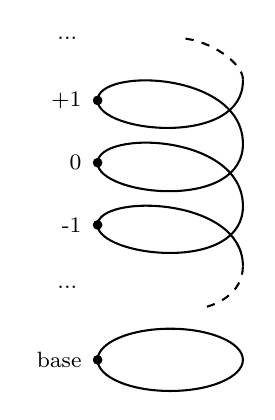
\begin{tikzpicture}[x=0.75pt,y=0.75pt,yscale=-1,xscale=1,roundnode/.style={circle, fill=black, inner sep=0pt, minimum size=3.5pt}]
  %uncomment if require: \path (0,300); %set diagram left start at 0, and has height of 300
  \node[roundnode, label=west:{\footnotesize{\con{base}}}] (B) at (40,165) {} ;
  \node[label=west:{\footnotesize{\anum{...}}}] (B) at (40,10) {} ;
  \node[roundnode, label=west:{\footnotesize{\anum{+1}}}] (B) at (40,40) {} ;
  \node[roundnode, label=west:{\footnotesize{\anum{0}}}] (B) at (40,70) {} ;
  \node[roundnode, label=west:{\footnotesize{\anum{-1}}}] (B) at (40,100) {} ;
  \node[label=west:{\footnotesize{\anum{...}}}] (B) at (40,130) {} ;
  
  %Shape: Ellipse [id:dp5332003998369562] 
  \draw   (40,165) .. controls (40,156.72) and (55.67,150) .. (75,150) .. controls (94.33,150) and (110,156.72) .. (110,165) .. controls (110,173.28) and (94.33,180) .. (75,180) .. controls (55.67,180) and (40,173.28) .. (40,165) -- cycle ;
  %Curve Lines [id:da36749341448547557] 
  \draw    (110,30) .. controls (110.83,62.83) and (40.17,55.83) .. (40,40) .. controls (39.83,24.17) and (108.67,25.83) .. (110,60) .. controls (111.33,94.17) and (39.67,85.83) .. (40,70) .. controls (40.33,54.17) and (108.67,55.83) .. (110,90) .. controls (111.33,124.17) and (39.83,115.17) .. (40,100) .. controls (40.17,84.83) and (110.33,86.17) .. (110,120) ;
  %Curve Lines [id:da7416045578170326] 
  \draw  [dash pattern={on 3pt off 3pt}]  (110,30) .. controls (110.33,22.33) and (94.33,10.83) .. (80,10) ;
  %Curve Lines [id:da8787470643619226] 
  \draw  [dash pattern={on 3pt off 3pt}]  (110,120) .. controls (109.83,133.33) and (96.83,138.83) .. (90,140) ;

  \end{tikzpicture}
  \caption{Graphical representation of the \func{helix} as a dependent type on \func{S¹}. 
    A copy of the integers sits over \con{base}, and the type equivalence corresponding 
    to the successor function sits over \con{loop}.}
\end{marginfigure}
% 
By applying \func{ua} we then get a nontrivial
equality/path from \func{Int} to \func{Int} that we call
\func{sucPathInt}. Using this we can define:
%
\ExecuteMetaData[chapters/literate-agda/Circle.tex]{windings1}

Applying the \func{winding} function to an element of \func{ΩS¹} will
compute its winding number. For example, we can compute the winding
numbers $+3$ and $-1$ as follows:
%
\ExecuteMetaData[chapters/literate-agda/Circle.tex]{exwindings1}

The term \con{negsuc} \var{n} represents the number $- (n+1)$, so that
\con{negsuc} \anum{0} is indeed $-1$. Note that none of these examples
would have reduced to a numeral in axiomatic HoTT as they would have been stuck
on transporting along \func{ua}. The proofs of these would hence not
be proved by \func{refl}, but rather by manually rewriting with the
postulated computation rules for univalence.

In order to prove that \func{ΩS¹} \ \func{≡}\ \func{Int} we just have
to define an inverse function to \func{winding}. This is easily done
via pattern matching.
%
\ExecuteMetaData[chapters/literate-agda/Circle.tex]{loopn}

% and we call the resulting function \func{loopn} :
% \func{Int} → \func{ΩS¹}.

It is then easy to prove that the \func{winding} number of an $n$-fold
\con{loop} is $n$.
%
\ExecuteMetaData[chapters/literate-agda/Circle.tex]{windingloopn}

Note that we parameterize by \var{i} in the second and fourth case of
\func{winding-loopn}. The reason for this is that we are constructing
an element of \func{≡}, i.e. a function out of \func{I}. This use of
interval variables hence lets us inline \func{cong}/\func{ap}.

However, when trying to prove the other composition one quickly
realizes that it is not as easy as there is no direct induction
principle for \func{ΩS¹}.
Luckily there is an ingenious solution to
this offered by HoTT in the form of the \emph{encode-decode method}
\sidecite[][Section 8.9]{HottBook13}. The trick is to generalize the
\func{loopn} and \func{winding} functions as follows:
%
\ExecuteMetaData[chapters/literate-agda/Circle.tex]{encode}
% TODO: There is a bit much space here. Fix if necessary.
\ExecuteMetaData[chapters/literate-agda/Circle.tex]{decode}

Note that \func{decode} \con{base} is \func{loopn} and that
\func{encode} \con{base} is \func{winding} definitionally. The
\con{loop} case of \func{decode} is not too difficult to define cubically,
but it does involve a few lines of path algebra. We chose to omit
it from our exposition to avoid getting sidetracked, but the interested
reader can find it in appendix \ref{sec:ap:loop-circle}.
% 
The main reason for generalizing the functions as above
is that we can now use path induction to prove the following:
%
\ExecuteMetaData[chapters/literate-agda/Circle.tex]{decodeEncode}

The special case \func{decodeEncode} \con{base} proves the desired
composition, i.e. that
$\func{loopn}~(\func{winding}~\var{x})~\func{≡}~\var{x}$ for all
\var{x} : \func{ΩS¹}. We may then package this up to get the desired
equality:
%
\ExecuteMetaData[chapters/literate-agda/Circle.tex]{omegas1}

By combining this result with the equality between the torus and two
circles we obtain:
% 
\sideremark{The loop space of a cartesian product of two types is the cartesian 
  product of the individual loop spaces, since the loop space is more or less a
  function type.}
%
\ExecuteMetaData[chapters/literate-agda/Torus.tex]{omegatorusintint}

% Once again we omit the definition due to space constraints.
It is now possible to transport along this equality to compute winding
numbers on the torus. However, this will not result in the most
efficient function possible and we can easily write a more direct
function for computing these numbers as follows.
%
\ExecuteMetaData[chapters/literate-agda/Torus.tex]{windingTorus}

Just like \func{winding} this function also computes as expected:
%
\ExecuteMetaData[chapters/literate-agda/Torus.tex]{exwindingTorus}

\section{Suspension, Spheres and Pushouts}
\label{sec:susp-pushout}

In this section we discuss various results about spheres, culminating
in two proofs that the 3-dimensional sphere is equal to the join of
two circles --- a result that we will need when computing the total
space of the Hopf fibration later on. On the way to this result we
introduce the pushout and join HITs. We also prove some useful results
about these, including the ``$3 \times 3$ lemma'' for pushouts and
associativity of the join.

\subsection{Suspension}
\label{sec:susp}

The suspension of a type \var{A} is built from two distinguished
points \con{north} and \con{south}, along with a path from \con{north}
to \con{south} for every point of \var{A} (and a homotopy square for
every path in \var{A}, etc.):
%
\ExecuteMetaData[chapters/literate-agda/Susp.tex]{susp}

The suspension of a type $A$ is depicted below.
% 
%\tikzset{every picture/.style={line width=0.75pt}} %set default line width to 0.75pt
\begin{figure}[H]
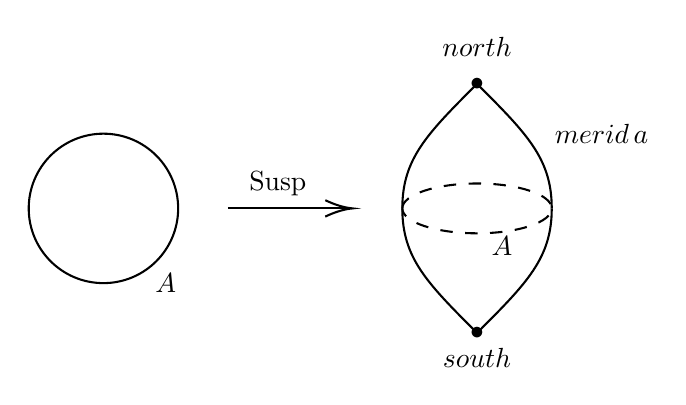
\begin{tikzpicture}[x=0.75pt,y=0.75pt,yscale=-1.2,xscale=1.2]
  %Shape: Circle
  \draw  [line width=0.75] (10,60) .. controls (10,43.43) and (23.43,30) .. (40,30) .. controls (56.57,30) and (70,43.43) .. (70,60) .. controls (70,76.57) and (56.57,90) .. (40,90) .. controls (23.43,90) and (10,76.57) .. (10,60) -- cycle ;
  \node (A1) at (65, 90) {$A$};
%  \node (A1) at (55, 45) {$A$};
  %Arrow
  \draw [line width=0.75] (90,60) -- (138,60) ;
  \draw [shift={(140,60)}, rotate = 180] [color={rgb, 255:red, 0; green, 0; blue, 0 }  ][line width=0.75]    (10.93,-3.29) .. controls (6.95,-1.4) and (3.31,-0.3) .. (0,0) .. controls (3.31,0.3) and (6.95,1.4) .. (10.93,3.29)   ;
  \node (S) at (110,50) {\func{Susp}};
  %Shape: Ellipse
  \draw  [line width=0.75][dash pattern={on 4.5pt off 4.5pt}] (160,60) .. controls (160,54.48) and (173.43,50) .. (190,50) .. controls (206.57,50) and (220,54.48) .. (220,60) .. controls (220,65.52) and (206.57,70) .. (190,70) .. controls (173.43,70) and (160,65.52) .. (160,60) -- cycle ;
  \node (A2) at (200,75) {$A$};
  %Curve Lines
  \draw [line width=0.75] (160,60) .. controls (160,80) and (170,90) .. (190,110) ;
  \draw [line width=0.75] (190,110) .. controls (210,90) and (220,80) .. (220,60) ;
  \draw [line width=0.75] (160,60) .. controls (160,40) and (170,30) .. (190,10) ;
  \draw [line width=0.75] (190,10) .. controls (210,30) and (220,40) .. (220,60) ;
  %Poles
  \node (N) at (190,10) {$\bullet$};
  \node (N2) at (190,-5) {$\con{north}$};
  \node (S) at (190,110) {$\bullet$};
  \node (S2) at (190,120) {$\con{south}$};
  %Meridians
  \node (M) at (240,30) {$\con{merid}\,\var{a}$};
\end{tikzpicture}
\caption{The suspension of a circle is a a sphere}
\end{figure}

In this drawing $A$ is a circle, in which case the suspension of \( A \) is a
sphere. This construction generalizes well, and we can define the higher dimensional spheres as
iterated suspensions starting from the booleans.
% 
\sideremark{Remark that the regular sphere is considered 2-dimensional, even 
  though it is the unit sphere of 3-dimensional space. 
  % 
  This is because the dimension refers to the number of parameters needed to 
  (locally) describe a point on the object.}
%
\ExecuteMetaData[chapters/literate-agda/Susp.tex]{nsphere}

We may now prove that our initial definition for the circle is equal
to the suspension of the booleans.

\begin{lemma} \label{lem:susps1}
  The (\anum{1})\func{-sphere} is equal to the circle \func{S¹}.
\end{lemma}
\begin{proof}
  We will prove this by constructing an isomorphism and then
  converting it to an equality using univalence. We first define a map
  from (\anum{1})\func{-sphere} to \( \func{S¹} \) in the following
  way, collapsing \( \con{merid}\,\con{false} \) to \( \con{base} \):
  %
  \ExecuteMetaData[chapters/literate-agda/Susp.tex]{s2c}

  In the other direction, we use composition to go around the
  (\anum{1})\func{-sphere} in one go.
  %
  \ExecuteMetaData[chapters/literate-agda/Susp.tex]{c2s}

  To construct the first canceling homotopy, we have to find a
  homotopy between \func{s2c}\,(\func{c2s}\,\con{loop}) =
  \con{loop}\,\func{∙}\,\func{refl} and \con{loop}. This is proved in
  one of the lemmas in the cubical library that says that \func{refl}
  is the right unit for \func{\_∙\_}.
  %
  \ExecuteMetaData[chapters/literate-agda/Susp.tex]{s2c-c2s}

  The second homotopy is slightly more involved.  After going back and
  forth, \( \con{merid}\ \con{false} \) has been collapsed to the
  \con{north} pole, while \( \con{merid}\ \con{true} \) has been
  stretched to go around the whole circle. As such, we need to move
  the \con{south} pole back into place along \(
  \con{merid}\ \con{false} \), and deform the two meridians
  accordingly:
  %
  \ExecuteMetaData[chapters/literate-agda/Susp.tex]{c2s-s2c}

  We need \func{h1} to be a homotopy from the constant path at
  \con{north} to the original path \( \con{merid}\ \con{false} \),
  such that the restriction to \( (\var{i} = \con{i1}) \) matches
  \( \con{merid}\ \con{false}\ \var{j} \) and the restriction to
  \( (\var{i} = \con{i0}) \) matches \con{north}. This is easily
  achieved using \func{\_∧\_}:
  %
  \ExecuteMetaData[chapters/literate-agda/Susp.tex]{h1}

  \sloppy
  On the other hand, \func{h2} has to be a homotopy from
  \( \con{merid}\ \con{true}\ \func{∙}\ \con{merid}\ \con{false}\ \func{⁻¹} \)
  to \( \con{merid}\ \con{true} \), with the same condition on the
  restrictions to \( (\var{i} = \con{i0}) \) and
  \( (\var{i} = \con{i1}) \). We can do that using \func{hcomp} to paste
  several homotopies together:

  \ExecuteMetaData[chapters/literate-agda/Susp.tex]{h2}

  The composition can be pictured as follows, showing both the outer
  edge constraints and the inner faces we used:

  \begin{figure}[H]
    \begin{tikzpicture}[xscale=1,yscale=1]
      \draw [thin, -latex'] (0.9,0.9) -- (2.1,0.9) ;
      \draw [thin, -latex'] (2.1,0.9) -- (2.1,2.1) ;
      \draw [thin, -latex'] (0.9,2.1) -- (2.1,2.1) ;
      \draw [thin, -latex'] (0.9,0.9) -- (0.9,2.1) ;

      \draw [thin, -latex'] (0.9,0.9) -- (0,0) ;
      \draw [thin, -latex'] (0.9,2.1) -- (0,3) ;
      \draw [thin, -latex'] (2.1,0.9) -- (3,0) ;
      \draw [thin, -latex'] (2.1,2.1) -- (3,3) ;

      \draw [thin, -latex'] (3,0) -- (3,3) ;
      \draw [thin, -latex', dashed] (0,0) -- (3,0) ;
      \draw [thin, -latex'] (0,3) -- (3,3) ;
      \draw [thin, -latex'] (0,0) -- (0,3) ;

      %% \node (top) at (1,-0.25) {\footnotesize \( \con{inl}\,(\con{push}\,(\field{f12}\, a)\, i) \)};
      %% \node (bot) at (1,2.25) {\footnotesize \( \con{inr}\,(\con{push}\,(\field{f32}\, a)\, i) \)};

      %% % is this bad practice? I dont know how local this change is.
      \setlength{\baselineskip}{8pt}
      %% \node[align=left] at (-1.2,1) {\footnotesize{\( \func{A□0-A○□} \)}\\\quad\footnotesize{\( (\func{f□1}\, (\con{push}\, a\, j)) \)}};
      %% \node[align=left] (rgt) at (3.2,1) {\footnotesize \( \func{A□4-A○□} \)\\\quad\footnotesize{\( \,(\func{f□3}\, (\con{push}\, a\, j)) \)}};

      \node (s2) at (0.45, 1.5) {\footnotesize \con{north}};
      \node[align=center] (s3) at (2.55, 1.5) {\footnotesize{\con{merid}} \\ \footnotesize{\( \con{false} \)} \\ \footnotesize{\( (j\ \func{∨}\ \func{\textasciitilde} k) \)} };
      \node[align=center] (s4) at (1.5, 2.55) {\footnotesize{\con{merid}} \\ \footnotesize{\( \con{true}\ i \)}};
      \node[align=center] (s5) at (1.5, 1.5) {\footnotesize{\con{merid}} \\ \footnotesize{\( \con{true}\ i \)}};

      \node [anchor=south] at (1.5,3) {\footnotesize \( \con{merid}\ \con{true}\ i \)};
      \node [anchor=north, rotate=90] at (3,1.5) {\footnotesize \( \con{merid}\ \con{false}\ j \)};
      \node [anchor=south, rotate=90] at (0,1.5) {\footnotesize \( \con{north}\ \)};
      \node [anchor=north] at (1.5,0) {\footnotesize  \( (\con{merid}\ \con{true}\ \func{∙}\ \con{merid}\ \con{false}\ \func{⁻¹})\ i \)};

      \draw [thin,->] (-2.5,0.5) -- (-2.5,1.3) ;
      \draw [thin,->] (-2.5,0.5) -- (-1.7,0.5) ;
      \draw [thin,->] (-2.5,0.5) -- (-2.9,0.15) ;
      \node [anchor=north] (x) at (-1.7, 0.5) {\footnotesize \( i \)};
      \node [anchor=west] (y) at (-2.5, 1.3) {\footnotesize \( j \)};
      \node [anchor=south] (z) at (-2.9, 0.15) {\footnotesize \( k \)};
      %\draw [thin,->] (-3.5,0) -- (-3.2,0.3) ;
    \end{tikzpicture}
    \caption{Using a two-dimensional \func{hcomp} to build a homotopy. The drawing represents
      an open box viewed from the top.}
  \end{figure}

  The \( (\var{j} = \con{i0}) \) face of the open cube matches the square used
  to define the composition
  \( \con{merid}\ \con{true}\ \func{∙}\ \con{merid}\ \con{false}\ \func{⁻¹} \)
  --- this breaks the composition into \func{refl},
  \( \con{merid}\ \con{true} \), and
  \( \con{merid}\ \con{false}\ \func{⁻¹} \) on the inner edges.
  Thus, we use the \( (\var{i} = \con{i1}) \) face to retract the
  \( \con{merid}\ \con{false}\ \func{⁻¹} \) part into the \con{south}
  pole, using a connection. The other faces are just constant in
  directions \( \var{j} \) and \( \var{k} \). From there, \func{hcomp} provides
  us with the front face of the cube, which is the homotopy we need.

  This completes the definition of \func{c2s-s2c}, providing us with
  an isomorphism than can be converted into an equality with
  \func{ua}.
  %% \loic{This is a bit difficult to follow. I can add details, but then
  %%   again this is not the focus of the paper...}  \anders{As you are
  %%   showing quite a bit more complicated hcomp's later it might be
  %%   good to explain this one in detail. Maybe we can drop some details
  %%   later.}  This gives use the desired isomorphism between the
  %% (\anum{1})\func{-sphere} and \func{S¹}, and thus an equality thanks
  %% to univalence.
\end{proof}

Inspired by the direct definition of \func{S¹} we can also give direct
definitions of some higher spheres, for example \func{S²} and
\func{S³} are defined as follows.
%
\ExecuteMetaData[chapters/literate-agda/Susp.tex]{s2}
% \anders{There is no need to use PathP here, but I think I only
%   introduced Path as \func{≡}}

As expected we can prove that these are equal to the definitions using
iterated suspensions. The proof of this lemma is very similar to the
one of \cref{lem:susps1} so we omit it.
%
\begin{lemma} \label{lem:susps23}
  The (\anum{2})\func{-sphere} is equal to \func{S²} and the
  (\anum{3})\func{-sphere} is equal to \func{S³}.
\end{lemma}

One might wonder if we can also give a direct definition of
\func{S$^n$} in a similar fashion and prove that it is equal to the
(\anum{n-1})\func{-sphere}. However, it is currently not possible to
write the higher constructor corresponding to \con{surfₙ} in \CubicalAgda 
as this kind of HIT is not supported by any of the proposed
schemas for cubical HITs~\sidecite{CHM,CavalloHarper19}. Interestingly it
is in fact possible to \emph{postulate} this HIT in HoTT or cubical
type theory, and prove properties about it --- for instance
\sidecitet{pinsn} prove that $\pi_n(\Sp^n) = \ZZ$ using this direct
definition.

\subsection{Pushouts and the 3 × 3 Lemma}
\label{sec:pushout}

Suppose we are given a span of types, consisiting in three types and two functions:

\begin{center}
\begin{tikzpicture}[xscale=1.5,yscale=2]
  \node (B) at (0,0) {\var{B}};
  \node (A) at (1,0) {\var{A}};
  \node (C) at (2,0) {\var{C}};
  \path[thin,->,>=angle 90]
  (A) edge node[above]{\footnotesize \var{f}} (B)
  (A) edge node[above]{\footnotesize \var{g}} (C);
\end{tikzpicture}
\end{center}

Then the homotopical pushout of this span is a type that contains both
a copy of \var{B} and a copy of \var{C}, and a path identifying
\var{f}\,\var{a} and \var{g}\,\var{a} for every \var{a} in \var{A}.
It can be defined as a HIT in the following way.
% 
\sideremark{Homotopy pushouts are an instance of a \emph{homotopy colimit},
  the adequate notion of colimits when morphisms are defined up to a 
  deformation.}
% 

\ExecuteMetaData[chapters/literate-agda/Pushout.tex]{pushout}

A generic homotopical pushout is illustrated below: it consists of an
embedded copy of \var{B} and \var{C}, and a copy of
\( \var{A} \times \func{I} \) whose ends have been identified with
corresponding points in \var{B} and \var{C} according to \var{f} and
\var{g}.

\begin{figure}[H]
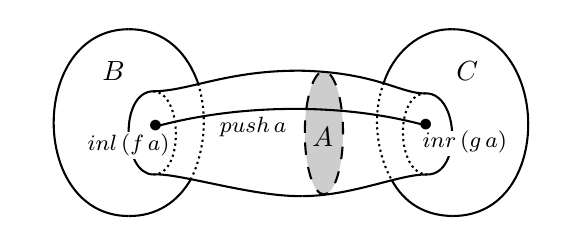
\begin{tikzpicture}[x=0.75pt,y=0.75pt,yscale=-1,xscale=1.2]

%Shape: Ellipse
  %\draw  [line width=0.75][fill={rgb, 255:red, 205; green, 205; blue, 205 }  ,fill opacity=1 ][dash pattern={on 4.5pt off 4.5pt}] (100,70.2) .. controls (100,53.52) and (104.48,40) .. (110,40) .. controls (115.52,40) and (120,53.52) .. (120,70.2) .. controls (120,86.88) and (115.52,100.4) .. (110,100.4) .. controls (104.48,100.4) and (100,86.88) .. (100,70.2) -- cycle ;
\draw  [line width=0.75][fill={rgb, 255:red, 205; green, 205; blue, 205 }  ,fill opacity=1 ][dash pattern={on 4.5pt off 4.5pt}] (110.76,69.92) .. controls (110.76,53.54) and (114.2,40.26) .. (118.43,40.26) .. controls (122.66,40.26) and (126.1,53.54) .. (126.1,69.92) .. controls (126.1,86.31) and (122.66,99.59) .. (118.43,99.59) .. controls (114.2,99.59) and (110.76,86.31) .. (110.76,69.92) -- cycle ;


%Curve Lines
\draw  [line width=0.75] (145.68,92.76) .. controls (150.68,103.56) and (158.68,109.76) .. (170,110) ;
\draw  [line width=0.75] (40,110) .. controls (51.27,110.18) and (59.93,103.07) .. (65.04,92.18) ;
\draw  [line width=0.75] (49.85,49.9) .. controls (64.18,49.93) and (79.83,39.53) .. (110,40) ;
\draw  [line width=0.75] (50,90) .. controls (59.83,89.03) and (90.18,100.93) .. (109.85,100.4) ;
\draw  [line width=0.75] (110,40) .. controls (140.33,41.03) and (149.68,51.43) .. (159.35,50.9) ;
\draw  [line width=0.75] (109.85,100.4) .. controls (129.68,100.43) and (149.33,89.53) .. (160,90) ;
\draw  [line width=0.75] (50,90) .. controls (37.3,89.9) and (36.15,50.3) .. (49.85,49.9) ;
\draw  [line width=0.75] (159.35,50.9) .. controls (172.85,50.9) and (173.8,89.9) .. (160,90) ;
\draw  [line width=0.75] (40,20) .. controls (55.04,19.94) and (63.93,32.17) .. (67.93,46.17) ;
\draw  [line width=0.75] (40,20) .. controls (-0.1,20.24) and (-0.1,109.91) .. (40,110) ;
\draw  [line width=0.75] (170,20) .. controls (209.85,20.27) and (211.35,110.27) .. (170,110) ;
\draw  [line width=0.75] (170,20) .. controls (156.28,19.76) and (146.08,32.36) .. (142.48,45.76) ;
\draw  [line width=0.75] (50.85,66.9) .. controls (82.85,56.4) and (124.85,54.9) .. (159.35,66.4) ;

\node (push) at (90,67) {\footnotesize \( \con{push}\,\var{a} \)};
\node (st) at (50.85,66.9) {\( \bullet \)};
\node [fill=white,inner sep=1,text height=6] (stl) at (40,76) {\footnotesize \( \con{inl}\,(\var{f\,a}) \)};
\node (nd) at (159.35,66.4) {\( \bullet \)};
\node [fill=white,inner sep=1,text height=5] (ndl) at (175,75) {\footnotesize \( \con{inr}\,(\var{g\,a}) \)};

\node (B) at (34,40) {$\var{B}$};
\node (A) at (118,72) {$\var{A}$};
\node (C) at (176,40) {$\var{C}$};

%Curve Lines [id:da3249943688792978]
\draw  [line width=0.75][dash pattern={on 0.8pt off 1.25pt}]  (67.93,46.17) .. controls (72.23,63.27) and (69.93,80.4) .. (65.04,92.18) ;
\draw  [line width=0.75][dash pattern={on 0.8pt off 1.25pt}]  (49.85,49.9) .. controls (61.73,50.11) and (62.28,90.21) .. (50,90) ;
\draw  [line width=0.75][dash pattern={on 0.8pt off 1.25pt}]  (159.35,50.9) .. controls (146.65,50.8) and (147.3,89.9) .. (160,90) ;
\draw  [line width=0.75][dash pattern={on 0.8pt off 1.25pt}]  (142.48,45.76) .. controls (137.08,63.16) and (140.48,81.96) .. (145.68,92.76) ;
\end{tikzpicture}
\caption{The homotopical pushout of the span \( B {\longleftarrow} A {\longrightarrow} C \)}
\end{figure}
%% \anders{I'm still a bit confused by this drawing. For example
%%   $\con{inl} (f~a)$ is not in B... Is the pushout supposed to be the
%%   tube? It's also bad style to have pictures that are not mentioned
%%   anywhere in the text.}
%% \loic{The pushout is the whole thing. This is the general picture of
%%   a homotopy pushout (in any ``nice enough'' model cat, including
%%   cubical sets) : one embedded copy of \( B \), one embedded copy of
%%   \( C \), and a copy of \( A \times I \) with extremities glued along
%%   \( f \) and \( g \). How should I illustrate this? Just drop the
%%   picture altogether? I like pictures :(}
%% \anders{I like the picture as well. It just need some explanation in
%%   the text similar to what you have written in the comment.}

Pushouts can be used to construct various classical objects such as
suspensions, joins and many more---hence their importance.  For
instance, the suspension of a type \( A \) is the homotopical pushout
of the following span:

\begin{center}
\begin{tikzpicture}[xscale=1.5,yscale=2]
  \node (B) at (0,0) {\( 1 \)};
  \node (A) at (1,0) {\var{A}};
  \node (C) at (2,0) {\( 1 \)};
  \path[thin,->,>=angle 90]
  (A) edge (B)
  (A) edge (C);
\end{tikzpicture}
\end{center}
where \( 1 \) is the inductive type with only one constructor, and the
arrows are the unique maps to \( 1 \).

Since pushouts are so ubiquitous, it is not rare to deal with nested pushouts.
In this case, a lemma known as the \( 3 \times 3 \) lemma comes in very handy 
to rearrange expressions:
%% \loic{cite Brunerie, Finster?}
%% \anders{We do that later so probably fine like this here}
suppose we are given a double span of types

\begin{center}
\begin{tikzpicture}[xscale=2,yscale=-2]
  \node (A00) at (0,0) {\( \func{A00} \)};
  \node (A20) at (1,0) {\( \func{A20} \)};
  \node (A40) at (2,0) {\( \func{A40} \)};
  \node (A02) at (0,1) {\( \func{A02} \)};
  \node (A22) at (1,1) {\( \func{A22} \)};
  \node (A42) at (2,1) {\( \func{A42} \)};
  \node (A04) at (0,2) {\( \func{A04} \)};
  \node (A24) at (1,2) {\( \func{A24} \)};
  \node (A44) at (2,2) {\( \func{A44} \)};
  \path[thin,->,>=angle 90]
  (A20) edge node[fill=white]{\footnotesize \( \field{f10} \)} (A00)
  (A20) edge node[fill=white]{\footnotesize \( \field{f30} \)} (A40)
  (A22) edge node[fill=white]{\footnotesize \( \field{f12} \)} (A02)
  (A22) edge node[fill=white]{\footnotesize \( \field{f32} \)} (A42)
  (A24) edge node[fill=white]{\footnotesize \( \field{f14} \)} (A04)
  (A24) edge node[fill=white]{\footnotesize \( \field{f34} \)} (A44)
  (A02) edge node[fill=white]{\footnotesize \( \field{f01} \)} (A00)
  (A02) edge node[fill=white]{\footnotesize \( \field{f03} \)} (A04)
  (A22) edge node[fill=white]{\footnotesize \( \field{f21} \)} (A20)
  (A22) edge node[fill=white]{\footnotesize \( \field{f23} \)} (A24)
  (A42) edge node[fill=white]{\footnotesize \( \field{f41} \)} (A40)
  (A42) edge node[fill=white]{\footnotesize \( \field{f43} \)} (A44);
  \draw[-implies,thin,double distance=3pt] (0.65,0.35) -- (0.35,0.65);
  \node (H11) at (0.35,0.35) {\footnotesize \( \field{H11} \)};
  \draw[-implies,thin,double distance=3pt] (1.35,0.35) -- (1.65,0.65);
  \node (H31) at (1.65,0.35) {\footnotesize \( \field{H31} \)};
  \draw[-implies,thin,double distance=3pt] (0.65,1.65) -- (0.35,1.35);
  \node (H13) at (0.35,1.65) {\footnotesize \( \field{H13} \)};
  \draw[-implies,thin,double distance=3pt] (1.35,1.65) -- (1.65,1.35);
  \node (H33) at (1.65,1.65) {\footnotesize \( \field{H33} \)};
\end{tikzpicture}
\end{center}
% \anders{I don't understand the numbering. Why isn't the top line
%   $A_{00}$, $A_{10}$ and $A_{20}$, etc?}
% \loic{This numbering is due to Guillaume, in his thesis. He uses even
%   numbers for types so that the numbering of maps is more natural.}
where the \( \field{Hij} \) are homotopies ensuring the commutativity of
the diagram: for instance, \( \field{H11} \) is of type
\( \field{f10}\,\func{∘}\,\field{f21} \ \func{≡}\  \field{f01}\,\func{∘}\,\field{f12} \).
% \anders{Maybe write this equality point-free? (i.e. without
%   quantifying over x)}
% \loic{Sure, if we are fine with assuming composition is defined.}

Then, there are two canonical ways to build a type from this diagram
out of pushouts.
We can start by taking the pushouts of the three rows, to get
the following span
%
\begin{equation} \label{span1}
\begin{tikzpicture}[xscale=2,yscale=2]
  \node (B) at (0,0) {\( \func{A□0} \)};
  \node (A) at (1,0) {\( \func{A□2} \)};
  \node (C) at (2,0) {\( \func{A□4} \)};
  \path[thin,->,>=angle 90]
  (A) edge node[above]{\footnotesize \( \func{f□1} \)} (B)
  (A) edge node[above]{\footnotesize \( \func{f□3} \)} (C);
\end{tikzpicture}
\end{equation}
in which we write \( \func{A□0} \) for the pushout of the first row
\( \func{A00} \leftarrow \func{A20} \rightarrow \func{A40} \), 
\( \func{A□2} \) for the pushout of the second row and \( \func{A□4} \) 
for the pushout of the third row. The maps between them, \( \func{f□1}
\) and \( \func{f□3} \), are then defined using pattern matching as 
follows:
%
\ExecuteMetaData[chapters/literate-agda/Pushout.tex]{fx1}
%% \loic{Should I add more detail here?}
%% \anders{I think that if you add more explanations of the hcomp in
%%   \func{c2s-s2c} then you don't need any more details here as this one
%%   is simpler.}

Finally, we write \( \func{A□○} \) for the pushout of the span in
(\ref{span1}). 
% 
\sideremark{On a more abstract level, both \( \func{A□○} \) and 
  \( \func{A○□} \) are homotopy colimits of the \( 3\times3 \) diagram,
  and as such they ought to be equivalent.}
% 
Conversely, we could have started by taking the pushout
of the columns and then computed the pushout \( \func{A○□} \) of the
resulting ``horizontal'' span. The \( 3\times3 \) lemma for pushouts
then states that the results of these two constructions are equal.

\begin{lemma}{(\( 3\times3 \) lemma)}\label{3x3}
  The two pushouts \( \func{A□○} \) and \( \func{A○□} \) are equal.
\end{lemma}
\begin{proof}
In order to prove this we construct an isomorphism via pattern
matching and apply univalence. To define a map \( \func{A□○} \to
\func{A○□} \), we will first need maps for the two sides of our
pushout span:
%
\ExecuteMetaData[chapters/literate-agda/Pushout.tex]{forward-l}

The map \func{A□4-A○□} is defined analogously. Using these maps we
can define the first map between the total pushouts:
%
\ExecuteMetaData[chapters/literate-agda/Pushout.tex]{forward}
Note how we did not define a map \func{A□2-A○□} to handle the
\con{push} case, but instead proceeded via nested pattern matching.
The reason is that when \Agda checks boundary constraints, it does not
perform \( \eta \)-expansion on its own so we have to do it by hand in the
function definition.
%% \anders{This remark is very technical and Agda specific. Maybe drop if
%%   we run out of space?}
%% \loic{Agreed. Maybe a footnote?}
%% \anders{Maybe, let's see how we are doing with space.}
%% \anders{Actually I think this remark is fine to keep.}

Most cases boil down to swapping the constructors, but this
straightforward strategy will not be sufficient to handle the last
case.
To fill this hole, we need to construct a square inside \( \func{A○□} \) with a
prescribed boundary. The most natural guess would be
\( \con{push}\,(\con{push}\,a\,i)\,j \), but its boundary for
\( i = \con{i0} \) is
\( \con{push}\, (\con{inl}\, (\field{f21}\,a))\, j \), which is not
definitionally equal to the prescribed
\( \func{A□0-A○□} (\func{f□1}\, (\con{push}\, a\, j)) \).

In order to get the proper square, we will use \func{hcomp} to glue the four
squares $s1$--$s4$ around our candidate in order to ensure it matches
the dashed boundary:

\begin{figure}[H]
\begin{tikzpicture}[xscale=1,yscale=1]
  \draw [thin, -latex'] (0.6,0.6) -- (1.4,0.6) ;
  \draw [thin, -latex'] (1.4,0.6) -- (1.4,1.4) ;
  \draw [thin, -latex'] (0.6,1.4) -- (1.4,1.4) ;
  \draw [thin, -latex'] (0.6,0.6) -- (0.6,1.4) ;

  \draw [thin, -latex'] (0.6,0.6) -- (0,0) ;
  \draw [thin, -latex'] (0.6,1.4) -- (0,2) ;
  \draw [thin, -latex'] (1.4,0.6) -- (2,0) ;
  \draw [thin, -latex'] (1.4,1.4) -- (2,2) ;

  \draw [thin, -latex', densely dashed] (0,0) -- (2,0) ;
  \draw [thin, -latex', densely dashed] (2,0) -- (2,2) ;
  \draw [thin, -latex', densely dashed] (0,2) -- (2,2) ;
  \draw [thin, -latex', densely dashed] (0,0) -- (0,2) ;

  \node (top) at (1,-0.25) {\footnotesize \( \con{inl}\,(\con{push}\,(\field{f12}\, a)\, i) \)};
  \node (bot) at (1,2.25) {\footnotesize \( \con{inr}\,(\con{push}\,(\field{f32}\, a)\, i) \)};

  \setlength{\baselineskip}{8pt}
  \node[align=left] at (-1.2,1) {\footnotesize{\( \func{A□0-A○□} \)}\\\quad\footnotesize{\( (\func{f□1}\, (\con{push}\, a\, j)) \)}};
  \node[align=left] (rgt) at (3.2,1) {\footnotesize \( \func{A□4-A○□} \)\\\quad\footnotesize{\( \,(\func{f□3}\, (\con{push}\, a\, j)) \)}};

  \node (s1) at (1, 0.3) {\footnotesize s3};
  \node (s2) at (0.3, 1) {\footnotesize s1};
  \node (s3) at (1.7, 1) {\footnotesize s2};
  \node (s4) at (1, 1.7) {\footnotesize s4};
  \node (s5) at (1, 1) {\footnotesize s5};

  \draw [thin,->] (-3.5,0) -- (-3.5,0.8) ;
  \draw [thin,->] (-3.5,0) -- (-2.7,0) ;
  \node [anchor=north] (x) at (-2.7, 0) {\footnotesize \( i \)};
  \node [anchor=west] (y) at (-3.5, 0.8) {\footnotesize \( j \)};
  %\draw [thin,->] (-3.5,0) -- (-3.2,0.3) ;
\end{tikzpicture}
\caption{Using a two-dimensional hcomp to rectify the boundary of 
  \( \con{push}\,(\con{push}\,a\,i)\,j \)}
\end{figure}

Thus we now explain how to construct the squares $s1$--$s5$, in this order.

To construct $s1$, we start by simplifying the boundary condition 
\func{A□0-A○□} \( (\func{f□1}\, (\con{push}\, a\, j)) \), which reduces to
\( \func{A□0-A○□}\, (\func{hcomp}\, ...) \).
% 
Function application commutes with \func{hcomp}'s up to a homotopy, so \func{A□0-A○□} 
applied to the composition is homotopic to the composition of the images of the
paths. That is, we can find a square with the following boundary:
\begin{figure}[H]
\begin{tikzpicture}[xscale=1,yscale=1]
  \draw [thin, -latex'] (0.3,0.3) -- (1.7,0.3) ;
  \draw [thin, -latex'] (1.7,0.3) -- (1.7,1.7) ;
  \draw [thin, -latex'] (0.3,1.7) -- (1.7,1.7) ;
  \draw [thin, -latex'] (0.3,0.3) -- (0.3,1.7) ;

  \node (top) at (1,0.1) {\footnotesize{\( \func{A□0-A○□}\,(\con{push}\,(\field{f21}\, a)\,j) \)}};
  \node (bot) at (1,1.9) {\footnotesize{\( \func{A□0-A○□}\, (\func{hcomp}\, ...) \)}};
  \setlength{\baselineskip}{8pt}
  \node[align=left] (lft) at (-1,1) {\footnotesize{\( \func{A□0-A○□} \)}\\\quad\footnotesize{\( (\con{inl}\, (\field{H11}\,a\,(\func{\textasciitilde} i))) \)}};
  \node[align=left] (rgt) at (3,1) {\footnotesize{\( \func{A□0-A○□} \)}\\\quad\footnotesize{\( (\con{inl}\, (\field{H31}\,a\,(\func{\textasciitilde} i))) \)}};

  \draw [thin,->] (-3.5,0.2) -- (-3.5,1) ;
  \draw [thin,->] (-3.5,0.2) -- (-2.7,0.2) ;
  \node [anchor=north] (x) at (-2.7, 0.2) {\footnotesize \( j \)};
  \node [anchor=west] (y) at (-3.5, 1) {\footnotesize \( i \)};
\end{tikzpicture}
\caption{Constructing the square \( s1 \)}
\end{figure}
Once rotated counter-clockwise, we can use this square for $s1$.
We proceed similarly for the square $s2$. 
% 
For the three remaining squares, we are left with the following boundary:
%
\begin{figure}[H]
\begin{tikzpicture}[xscale=1,yscale=1]
  \draw [thin, -latex'] (0.6,0.6) -- (1.4,0.6) ;
  \draw [thin, -latex'] (1.4,0.6) -- (1.4,1.4) ;
  \draw [thin, -latex'] (0.6,1.4) -- (1.4,1.4) ;
  \draw [thin, -latex'] (0.6,0.6) -- (0.6,1.4) ;

  \draw [thin, -latex'] (0,0) -- (0.6,0.6);
  \draw [thin, -latex'] (0.6,1.4) -- (0,2) ;
  \draw [thin, -latex'] (2,0) -- (1.4,0.6) ;
  \draw [thin, -latex'] (1.4,1.4) -- (2,2) ;

  \draw [thin, -latex'] (0,0) -- (2,0) ;
  \draw [thin, -latex'] (0,2) -- (2,2) ;

  \node (top) at (1,-0.25) {\footnotesize \( \con{inl}\,(\con{push}\,(\field{f12}\, a)\, i) \)};
  \node (bot) at (1,2.25) {\footnotesize \( \con{inr}\,(\con{push}\,(\field{f32}\, a)\, i) \)};
  \node (lft) at (-0.6,1) {\footnotesize \( \con{push}\, (\con{inl}\, (\field{f21}\,a))\, j \)};
  \node (lft1) at (-0.9,0.4) {\footnotesize \( \con{inl}\, (\con{inl}\, (\field{H11}\,a\,j)) \)};
  \node (lft2) at (-0.9,1.6) {\footnotesize \( \con{inr}\, (\con{inl}\, (\field{H31}\,a\, j)) \)};
  \node (rgt) at (2.6,1) {\footnotesize \( \con{push}\, (\con{inr}\, (\field{f21}\,a))\, j \)};
  \node (rgt1) at (2.9,0.4) {\footnotesize \( \con{inl}\, (\con{inr}\, (\field{H13}\,a\, j)) \)};
  \node (rgt2) at (2.9,1.6) {\footnotesize \( \con{inr}\, (\con{inr}\, (\field{H33}\,a\, j)) \)};

  \node (s1) at (1, 0.3) {\footnotesize s3};
  \node (s4) at (1, 1.7) {\footnotesize s4};
  \node (s5) at (1, 1) {\footnotesize s5};

  \draw [thin,->] (-3.5,0) -- (-3.5,0.8) ;
  \draw [thin,->] (-3.5,0) -- (-2.7,0) ;
  \node [anchor=north] (x) at (-2.7, 0) {\footnotesize \( i \)};
  \node [anchor=west] (y) at (-3.5, 0.8) {\footnotesize \( j \)};
\end{tikzpicture}
\caption{Remaining boundary}
\end{figure}

%% \loic{should I go 3D with the axes? when writing the actual
%%   \func{hcomp}, there is a \( k \) dimension but it is impractical
%%   to tikz...}
%% \anders{It might be nice to have at least tips on the arrows in the diagram}
%% \loic{I tried it, but I'm not very enthusiastic about them. What do you think?}
%% \anders{It doesn't look good when the tips overlap. Apart from that I think they are helpful}

Just like before, we can use the functoriality of \con{inl} to get
a square with the following boundary:

\begin{figure}[H]
\begin{tikzpicture}[xscale=1,yscale=1]
  \draw [thin, -latex'] (0.3,0.3) -- (1.7,0.3) ;
  \draw [thin, -latex'] (1.7,0.3) -- (1.7,1.7) ;
  \draw [thin, -latex'] (0.3,1.7) -- (1.7,1.7) ;
  \draw [thin, -latex'] (0.3,0.3) -- (0.3,1.7) ;

  \setlength{\baselineskip}{10pt}
  \node (top) at (1,0.1) {\footnotesize{\( \con{inl}\,(\con{push}\,(\field{f12}\, a)\,i) \)}};
  \node[align=center] (bot) at (1,2.1) {\footnotesize{\( \con{inl}\,(\func{f1□}\, (\con{push}\, a\, i)) \)}\\\footnotesize{\( = \con{inl}\,(\func{hcomp}\,...) \)}};
  \node (lft) at (-0.8,1) {\footnotesize{\( \con{inl}\, (\con{inl}\, (\field{H11}\,a\,j)) \)}};
  \node (rgt) at (2.8,1) {\footnotesize{\( \con{inl}\, (\con{inr}\, (\field{H13}\,a\,j)) \)}};

  \draw [thin,->] (-3.5,0.2) -- (-3.5,1) ;
  \draw [thin,->] (-3.5,0.2) -- (-2.7,0.2) ;
  \node [anchor=north] (x) at (-2.7, 0.2) {\footnotesize \( i \)};
  \node [anchor=west] (y) at (-3.5, 1) {\footnotesize \( j \)};
\end{tikzpicture}
\caption{The square \( s3 \)}
\end{figure}
We use this square for $s3$ and the appropriate analogue for $s4$. The
only square left to construct now is
%
\begin{figure}[H]
\begin{tikzpicture}[xscale=1,yscale=1]
  \draw [thin, -latex'] (0.6,0.6) -- (1.4,0.6) ;
  \draw [thin, -latex'] (1.4,0.6) -- (1.4,1.4) ;
  \draw [thin, -latex'] (0.6,1.4) -- (1.4,1.4) ;
  \draw [thin, -latex'] (0.6,0.6) -- (0.6,1.4) ;

  \node (top) at (1,0.4) {\footnotesize \( \con{inl}\,(\func{f1□}\, (\con{push}\, a\, i))\)};
  \node (bot) at (1,1.6) {\footnotesize \( \con{inr}\,(\func{f3□}\, (\con{push}\, a\, i))\)};
  \node (lft) at (-0.6,1) {\footnotesize \( \con{push}\, (\con{inl}\, (\field{f21}\,a))\, j \)};
  \node (rgt) at (2.6,1) {\footnotesize \( \con{push}\, (\con{inr}\, (\field{f21}\,a))\, j \)};

  \node (s5) at (1, 1) {\footnotesize s5};

  \draw [thin,->] (-3.5,0.5) -- (-3.5,1.3) ;
  \draw [thin,->] (-3.5,0.5) -- (-2.7,0.5) ;
  \node [anchor=north] (x) at (-2.7, 0.5) {\footnotesize \( i \)};
  \node [anchor=west] (y) at (-3.5, 1.3) {\footnotesize \( j \)};
\end{tikzpicture}
\caption{Remaining boundary for \( s5 \)}
\end{figure}
which we can fill with \( \con{push}\,(\con{push}\,a\,i)\,j \).
By combining these five squares using \func{hcomp} we can finally complete
our definition of \( \func{A□○} \to \func{A○□} \).

The opposite direction, \( \func{A○□} \to \func{A□○} \), is the same
up to a transposition of the \( 3\times3 \) span. The proofs that
these maps cancel are also similar, but the central fillers are more
difficult to illustrate as they require one more dimension. We refer
the interested reader to the formalization. By combining all of this
we obtain the desired equality between \( \func{A□○} \) and
\( \func{A○□} \).
\end{proof}

The formal proof of the $3 \times 3$ lemma is under $200$ lines of
code~(LOC) in \CubicalAgda. The
corresponding result in \texttt{HoTT-Agda} is about $3000$ LOC.
\sideremark{This number has been calculated by counting the number of lines 
  (excluding comments) in:
  \url{https://github.com/HoTT/HoTT-Agda/tree/master/theorems/homotopy/3x3}}
These numbers should of course be taken with a grain of salt as those
proofs are not self-contained and rely on other results in the
library. 
% 
Regardless, we believe that it is a reasonably good illustration of how having
HITs with definitional computation rules simplifies the path algebra.

%% We will also need the following auxiliary lemma about pushouts further on:
%% \begin{lemma}\label{pushoutId}
%%   The pushout of
%%   \begin{center}
%%     \begin{tikzpicture}[xscale=1.5,yscale=2]
%%       \node (B) at (0,0) {\var{A}};
%%       \node (A) at (1,0) {\var{A}};
%%       \node (C) at (2,0) {\var{C}};
%%       \path[thin,->,>=angle 90]
%%       (A) edge node[above]{\footnotesize \func{id}} (B)
%%       (A) edge node[above]{\footnotesize \var{g}} (C);
%%     \end{tikzpicture}
%%   \end{center}
%%   is equal to A.
%% \end{lemma}
%% \loic{Should I inline this in the proof of join associativity?}
%% \anders{Maybe, it could just be a short remark there.}

\subsection{The Join and \func{S³}}
\label{sec:join}

Another interesting example of a pushout is the join. 
% 
The main role of this construction in this chapter is to give us a
presentation of \func{S³} as the join of two circles, which will be
useful when proving that the total space of the Hopf fibration is
\func{S³}. However, this construction also has many other interesting
uses in HoTT as explored by \sidecitet{Rijke17}.

The join of two types \var{A} and \var{B} is built from one copy of
\var{A}, one copy of \var{B}, and a path from every \( a\,:\,A \) to
every \( b\,:\,B \).
%
\ExecuteMetaData[chapters/literate-agda/Join.tex]{join}

It is easy to see that \( \func{Join}\ A\ B \) can alternatively be
defined as the pushout of the following span---the inductive
definitions only differ by currying.
%
\begin{center}
\begin{tikzpicture}[xscale=2.5,yscale=2]
  \node (B) at (0,0) {\( A \)};
  \node (A) at (1,0) {\( A \times B\)};
  \node (C) at (2,0) {\( B \)};
  \path[thin,->,>=angle 90]
  (A) edge node[above]{\footnotesize \( \func{fst} \)} (B)
  (A) edge node[above]{\footnotesize \( \func{snd} \)} (C);
\end{tikzpicture}
\end{center}

We now proceed by proving a few lemmas relating joins and spheres.

\begin{lemma}\label{joinbool}
  \( \func{Join}\ \func{Bool}\ A \ \func{≡}\  \func{Susp}\ A \).
\end{lemma}
\begin{proof}
  In \func{Join}\ \func{Bool}\ \var{A} the two points \con{inr}\
  \con{true} and \con{inr}\ \con{false} play the role of \con{north}
  and \con{south}, with a path connecting them to every point
  \con{inl}\ \var{a}.
\end{proof}
%% \loic{Should this proof be left as an exercise, like in the HoTT book?
%%   It is roughly similar to
%%   \( \func{Susp}\ \func{Bool} \ \func{≡}\  \func{S¹} \) in size.}
%% \anders{I like this short proof, so let's keep it if we have space}

The proof of the following result is taken from \sidecitet[][Proposition
1.8.6]{Brunerie16}, as such we will only sketch it here.

\begin{lemma}\label{joinassoc}
  \func{Join} is associative:
  \[ \func{Join}\ A\ (\func{Join}\ B\ C) \ \func{≡}\ \func{Join}\
    (\func{Join}\ A\ B)\ C \]
\end{lemma}
\begin{proof}
  %% \anders{I would refactor this a bit by moving the remark attributing
  %%   the proof to Brunerie outside and then giving a quite compact
  %%   proof.}
  %% \loic{I don't quite understand what you mean, do you think this
  %%   proof is too long?}
  %% \anders{I mean that we can say above the proof that it is due to
  %%   Brunerie and the proof should then be very short or just a
  %%   reference to where it can be found in his thesis. There are no new
  %%   cubical ideas in it so I don't think it is worth spending too much
  %%   space on it. Maybe just ``Apply the 3x3 lemma to the the following
  %%   diagram ... where all the arrows are the obvious projections and
  %%   the homotopies are refl's'' would be sufficient. If something is
  %%   unclear it can be found in Brunerie's thesis.}

  One starts by applying the \(3 \times 3\) lemma to the following
  diagram.
  %
  \begin{center}
    \begin{tikzpicture}[xscale=2,yscale=-1.3]
      \node (A00) at (0,0) {\( \var{A} \)};
      \node (A20) at (1,0) {\( \var{A}\times\var{B} \)};
      \node (A40) at (2,0) {\( \var{B} \)};
      \node (A02) at (0,1) {\( \var{A}\times\var{C} \)};
      \node (A22) at (1,1) {\( \var{A}\times\var{B}\times\var{C} \)};
      \node (A42) at (2,1) {\( \var{B}\times\var{C} \)};
      \node (A04) at (0,2) {\( \var{A}\times\var{C} \)};
      \node (A24) at (1,2) {\( \var{A}\times\var{C} \)};
      \node (A44) at (2,2) {\( \var{C} \)};
      \path[thin,->,>=angle 90]
      (A20) edge (A00)
      (A20) edge (A40)
      (A22) edge (A02)
      (A22) edge (A42)
      (A24) edge (A04)
      (A24) edge (A44)
      (A02) edge (A00)
      (A02) edge (A04)
      (A22) edge (A20)
      (A22) edge (A24)
      (A42) edge (A40)
      (A42) edge (A44);
    \end{tikzpicture}
  \end{center}

  All of the arrows in the diagram are the obvious projections, and
  the homotopies are \func{refl}'s. One can then show that
  \( \func{A□○} \ \func{≡}\ \func{Join}\ (\func{Join}\ A\ B)\ C \),
  and that
  \( \func{A○□} \ \func{≡}\ \func{Join}\ A\ (\func{Join}\ B\ C) \),
  which implies the desired result.
\end{proof}

We now have all of the ingredients to relate \func{S³} and the
\func{Join} of two circles.

\begin{lemma}\label{joins1s1}
  \( \func{Join}\ \func{S¹}\ \func{S¹} \ \func{≡}\  \func{S³} \)
\end{lemma}
\begin{proof}
This is a composition of equalities we already proved.
\begin{align*}
  \func{Join}\ \func{S¹}\ \func{S¹} \
  & \func{≡}\ \func{Join}\ (\func{Susp}\ \func{Bool})\ \func{S¹}
  & (\ref{lem:susps1})\\
  & \func{≡}\ \func{Join}\ (\func{Join}\ \func{Bool}\ \func{Bool})\ \func{S¹}
  & (\ref{joinbool})\\
  & \func{≡}\ \func{Join}\ \func{Bool}\ (\func{Join}\ \func{Bool}\ \func{S¹})
  & (\ref{joinassoc})\\
  & \func{≡}\ \func{Susp}\ (\func{Susp}\ \func{S¹})
  & (\ref{joinbool})\\
  & \func{≡}\ \func{S³}
  &&\qedhere
\end{align*}
\end{proof}

The above proof is an elegant application of the \( 3\times3 \) lemma,
but it results in rather complicated maps between \func{Join}
\func{S¹} \func{S¹} and \func{S³}. 
% 
\sideremark{For details see the \redtt{} proof
  at:\\ \url{https://github.com/RedPRL/redtt/blob/master/library/cool/s3-to-join.red}}
% 
Evan Cavallo has found a more
direct cubical proof that \( \func{Join}\ \func{S¹}\ \func{S¹}
\ \func{≡}\ \func{S³} \) by simply defining the maps directly and
proving that they cancel.
% 
We have ported his proof to \CubicalAgda and the resulting
proof is very short ($\sim60$ LOC). However, the proofs that the maps
cancel require a $4$-dimensional(!) \func{hcomp} making it rather
difficult to visualize.

\section{The Hopf Fibration}
\label{sec:hopf}

In this section we define the Hopf 
fibration
\sideremark{Fibrations are a concept from classical topology 
  that encode a space that varies continuously over a base space. In 
  homotopy/cubical type theory, a fibration corresponds to a dependent type.}
\( \func{Hopf}\,:\,\func{S²} \to \func{Set} \). 
% 
The Hopf fibration is a dependent type over the sphere \func{S²} such that
\func{Hopf}~\con{base₂} is equal the circle \func{S¹} and such that the
total space \func{Σ}~(\var{x}~:~\func{S²})~.~\func{Hopf}~\var{x} is equal 
to \func{S³}. 
% 
This construction is useful because it allows us to compute homotopical properties 
of \func{S³} from the properties of \func{S²} and \func{S¹}.

We will define the Hopf fibration on \func{Susp}~\func{S¹} instead of 
\func{S²}, which does not really matter since both types are equal by
\cref{lem:susps23}.
Now, recall that \func{Susp}~\func{S¹} is the pushout of the span
\begin{center}
  \begin{tikzpicture}[xscale=1.5,yscale=2]
    \node (B) at (0,0) {\( 1 \)};
    \node (A) at (1,0) {\func{S¹}};
    \node (C) at (2,0) {\( 1 \)};
    \path[thin,->,>=angle 90]
    (A) edge (B)
    (A) edge (C);
  \end{tikzpicture}
\end{center}

Therefore, to define the function 
\( \func{Hopf}\,:\,\func{Susp}~\func{S¹} \to \func{Set} \) we must 
pick the image of the two poles, which will be \func{S¹}, and then
give a proof of \func{S¹}~\func{≡}~\func{S¹} indexed by \func{S¹}.
% 
By univalence, this amounts to defining a function 
\( f : \func{S¹} \to \func{S¹} \to \func{S¹} \) such that \( f~x \)
is an equivalence for all \( x : \func{S¹} \).

Now it happens that \( \func{S¹} \) has a natural group structure. 
This is easy to see if we think of \( \func{S¹} \) as the set of unitary 
complex numbers:
\[
e^{2i\pi \theta} \cdot e^{2i\pi \phi} = e^{2i\pi (\theta + \phi)}
\]
But of course, in cubical type theory \( \func{S¹} \) is defined as a HIT and 
not as the set of unitary complex numbers. 
The correct analogue of the complex product can be defined by pattern-matching 
as follows:
%
\ExecuteMetaData[chapters/literate-agda/Circle.tex]{rot}

The last case can be illustrated by the following diagram, where we
only annotated the edges and reduced the (constant) central face to
a tiny square:
%
\begin{figure}[H]
\begin{tikzpicture}[xscale=1,yscale=1]
  \draw [thin, -latex'] (1,1) -- (0,0) ;
  \draw [thin, -latex'] (1,1.4) -- (0,2.4) ;
  \draw [thin, -latex'] (1.4,1) -- (2.4,0) ;
  \draw [thin, -latex'] (1.4,1.4) -- (2.4,2.4) ;

  \draw [thin, -latex'] (0,0) -- (2.4,0) ;
  \draw [thin, -latex'] (2.4,0) -- (2.4,2.4) ;
  \draw [thin, -latex'] (0,2.4) -- (2.4,2.4) ;
  \draw [thin, -latex'] (0,0) -- (0,2.4) ;

  \draw [thin] (1,1) -- (1.4,1) ;
  \draw [thin] (1.4,1) -- (1.4,1.4) ;
  \draw [thin] (1,1.4) -- (1.4,1.4) ;
  \draw [thin] (1,1) -- (1,1.4) ;

  \node (top) at (1.2,-0.25) {\footnotesize \( \con{loop}\ j \)};
  \node (bot) at (1.2,2.65) {\footnotesize \( \con{loop}\ j \)};
  \node [rotate=90] (left) at (2.65,1.2) {\footnotesize \( \con{loop}\ k \)};
  \node [rotate=90] (right) at (-0.25,1.2) {\footnotesize \( \con{loop}\ k \)};
  \node [rotate=45, fill=white, inner sep=0,text height=6] (nw) at (0.55,0.55) {\footnotesize \( \con{loop}\ (\func{\textasciitilde} l) \)};
  \node [rotate=45, fill=white] (se) at (1.9,1.9) {\footnotesize \( \con{loop}\ l \)};
  \node [rotate=315, fill=white] (ne) at (1.9,0.5) {\footnotesize \( \con{base} \)};
  \node [rotate=315, fill=white] (sw) at (0.5,1.9) {\footnotesize \( \con{base} \)};

  \draw [thin,->] (-2.5,0.5) -- (-2.5,1.3) ;
  \draw [thin,->] (-2.5,0.5) -- (-1.7,0.5) ;
  \draw [thin,->] (-2.5,0.5) -- (-2.9,0.15) ;
  \node [anchor=north] (x) at (-1.7, 0.5) {\footnotesize \( j \)};
  \node [anchor=west] (y) at (-2.5, 1.3) {\footnotesize \( j \)};
  \node [anchor=south] (z) at (-2.9, 0.15) {\footnotesize \( l \)};
\end{tikzpicture}
\caption{Defining the product on the unit circle in cubical type theory}
\end{figure}

Indeed, our intuition from the complex numbers tells us that
\func{rot} (\con{loop}~\var{j}) (\con{loop}~\var{k}) is analogous to
\( e^{2i\pi (j + k)} \). So it is only natural that the \( j+k=1 \)
diagonal is constant at \con{base}, and the \( j = k \) diagonal
follows \con{loop} twice.
%% \anders{I'm still confused by the refl diagonal...}
%% \loic{refl diagonals correspond to \( i+j=1 \). It is only normal
%%   that they are constant at base since \( e^{2i\pi} \) is 1. Should I
%%   write \con{base} instead of \func{refl} ?}
%% \loic{Should I keep this figure?}
%% \anders{I don't understand the diagonals... The point imo is that we
%%   need a square that is loop on all sides. It is nice that this has such
%%   a direct cubical proof.}

This results in a binary operation on \func{S¹}, that we also write
as \( \_\func{*}\_ \) instead of \func{rot}. We can even get a
complete (higher) abelian group structure on \func{S¹}, with an
inverse operation that we call \func{inv}.
% -- the inverse being induced by path reversal.
%
\begin{lemma}
  % There is term \func{rotIsEquiv} of type\\ \( {(\var{a}:\func{S¹})
  % \to \func{isEquiv}\ (\func{rot}\ \var{a})} \).

  For every \var{x} : \func{S¹} we have an equivalence \func{rotEquiv}
  \var{x} : \func{S¹} \func{≃} \func{S¹} given by \func{rot} \var{x}.
\end{lemma}
\begin{proof}
  The inverse of \func{rot}~\var{x} is given by \func{rot}~(\func{inv}~\var{x}).
\end{proof}

We can now define the Hopf fibration using \func{ua} to convert \func{rot} into
an equality:
%
\ExecuteMetaData[chapters/literate-agda/Hopf.tex]{hopf}

In fact, we could have directly defined the Hopf fibration for
\func{S²} using \func{Glue} to glue the identity equivalence on three of the sides
of the 2-cell and the \func{rot} equivalence on the fourth side.
%
\ExecuteMetaData[chapters/literate-agda/Hopf.tex]{hopfs2}

However, it turns out that the version using \func{Susp} \func{S¹} is
easier to work with as we have more wiggle room with the
constructors.

We can now form the total space of the \func{Hopf} fibration
using a \func{Σ}-type:
\( \func{Σ}\ \func{Hopf} = \sum_{x : \func{Susp}\ \func{S¹}} \func{Hopf}\ x \).
Our main theorem can be stated as:
%
\begin{theorem} \label{thm:hopf}
  The total space of the Hopf fibration is \func{S³}, that is,
  \( \func{Σ}\ \func{Hopf}\ \func{≡}\ \func{S³} \).
\end{theorem}
\begin{proof} 
  We start by remarking that the space \func{Σ}~\func{Hopf} is the homotopical
  pushout of the following span:
  \begin{center}
    \begin{tikzpicture}[xscale=3,yscale=2]
      \node (B) at (0,0) {\func{S¹}};
      \node (A) at (1,0) {\( \func{S¹} \func{×}\ \func{S¹} \)};
      \node (C) at (2,0) {\func{S¹}};
      \path[thin,->,>=angle 90]
      (A) edge node[above]{\footnotesize \( \pi_2 \)} (B)
      (A) edge node[above]{\footnotesize \func{rot}} (C);
    \end{tikzpicture}
  \end{center}
  which can be seen by a straightforward unfolding of definitions.
  % 
  \sideremark{This change of variables could be avoided if we tailored our 
    definitions a bit better for this proof.
    This sort of irritating details is the downside of working with bare 
    cubical primitives instead of universal properties.}
  % 
  And with a change of variables, we can see \func{Σ}~\func{Hopf} as the homotopical 
  pushout of this alternative span, where 
  \func{rot'}~(\var{x}, \var{y}) = \func{rot}~(\func{inv}~\var{x})~\var{y}.
  \begin{center}
    \begin{tikzpicture}[xscale=3,yscale=2]
      \node (B) at (0,0) {\func{S¹}};
      \node (A) at (1,0) {\( \func{S¹} \func{×}\ \func{S¹} \)};
      \node (C) at (2,0) {\func{S¹}};
      \path[thin,->,>=angle 90]
      (A) edge node[above]{\footnotesize \func{rot'}} (B)
      (A) edge node[above]{\footnotesize \( \pi_2 \)} (C);
    \end{tikzpicture}
  \end{center}
  
  Now by \cref{joins1s1}, which states that
  \( \func{S³}\ \func{≡}\ \func{Join}\ \func{S¹}\ \func{S¹} \), it
  suffices to prove that
  \( \func{Σ}\ \func{Hopf}\ \func{≡}\ \func{Join}\ \func{S¹}\ \func{S¹} \). 
  But recall that \( \func{Join}\ \func{S¹}\ \func{S¹} \) is the
  pushout of the following span:
  \begin{center}
    \begin{tikzpicture}[xscale=3,yscale=2]
      \node (B) at (0,0) {\func{S¹}};
      \node (A) at (1,0) {\( \func{S¹} \func{×}\ \func{S¹} \)};
      \node (C) at (2,0) {\func{S¹}};
      \path[thin,->,>=angle 90]
      (A) edge node[above]{\footnotesize \( \pi_1 \)} (B)
      (A) edge node[above]{\footnotesize \( \pi_2 \)} (C);
    \end{tikzpicture}
  \end{center}

  To show that these two homotopical pushouts are isomorphic, we will describe 
  a span isomorphism (that is, a natural equivalence between these two spans),
  and translate it to a \CubicalAgda term.

  To go from \( \func{Join}\ \func{S¹}\ \func{S¹} \) to
  \( \func{Σ}\ \func{Hopf} \), we want to use the
  following natural equivalence:

  \begin{center}
    \begin{tikzpicture}[xscale=3,yscale=-2]
      \node (B1) at (0,0) {\func{S¹}};
      \node (A1) at (1,0) {\( \func{S¹} \func{×}\ \func{S¹} \)};
      \node (C1) at (2,0) {\func{S¹}};
      \node (B2) at (0,1) {\func{S¹}};
      \node (A2) at (1,1) {\( \func{S¹} \func{×}\ \func{S¹} \)};
      \node (C2) at (2,1) {\func{S¹}};

      \path[thin,->,>=angle 90]
      (A2) edge node[below]{\footnotesize \func{rot'}} (B2)
      (A1) edge node[above]{\footnotesize \( \pi_2 \)} (C1)
      (A1) edge node[above]{\footnotesize \( \pi_1 \)} (B1)
      (A2) edge node[below]{\footnotesize \( \pi_2 \)} (C2)
      (A1) edge node[fill=white, align=center]{\footnotesize \( (x, y) \mapsto \) \footnotesize \( (\func{rot'}\ x\ y, y) \)} (A2)
      (B1) edge node[left]{\footnotesize \( \func{id} \)} (B2)
      (C1) edge node[right]{\footnotesize \( \func{id} \)} (C2);
    \end{tikzpicture}
  \end{center}
  %\anders{Why not use \func{rot'} in the downwards mapsto?}

  which can be written as a map between pushouts as follows:
  %
  \ExecuteMetaData[chapters/literate-agda/Hopf.tex]{backward}

  Now our diagram says that the hole should be filled with \var{y},
  but the types do not match: \var{y} has type \func{S¹} while the hole expects 
  a term of type 
  \func{Glue}~\func{S¹}~(\symb{λ}~\{~(\var{i} = \con{i0}) → (\func{S¹},~\func{rotEquiv}\ (\func{rot'}\ (x , y)))\ ;\ (\var{i} = \con{i1}) → (\func{S¹},~\func{idEquiv}~\func{S¹})~\})\ \var{i}.
  To convert \var{y} into an inhabitant of this \func{Glue} type, we can use the 
  \func{glue} primitive as follows:
  % 
  \ExecuteMetaData[chapters/literate-agda/Hopf.tex]{backwardtwo}

  We supply it with a term \var{p}~\var{i} of type \func{S¹}, as well as a 
  partial term which coincides with \var{p}~\var{i} after application of the
  equivalences \func{rotEquiv} and \func{idEquiv}.
  % 
  The auxiliary lemma \func{lem-rot'} \var{x} \var{y} is defined by induction on
  \var{x} and \var{y}.

  Conversely, to go from \( \func{Σ}\ \func{Hopf} \) to
  \( \func{Join}\ \func{S¹}\ \func{S¹} \), we use the following
  natural isomorphism:
  %
  \begin{center}
    \begin{tikzpicture}[xscale=3,yscale=-2]
      \node (B1) at (0,0) {\func{S¹}};
      \node (A1) at (1,0) {\( \func{S¹} \func{×}\ \func{S¹} \)};
      \node (C1) at (2,0) {\func{S¹}};
      \node (B2) at (0,1) {\func{S¹}};
      \node (A2) at (1,1) {\( \func{S¹} \func{×}\ \func{S¹} \)};
      \node (C2) at (2,1) {\func{S¹}};

      \path[thin,->,>=angle 90]
      (A1) edge node[above]{\footnotesize \func{rot'}} (B1)
      (A1) edge node[above]{\footnotesize \( \pi_2 \)} (C1)
      (A2) edge node[below]{\footnotesize \( \pi_1 \)} (B2)
      (A2) edge node[below]{\footnotesize \( \pi_2 \)} (C2)
      (A1) edge node[fill=white, align=center]{\footnotesize \( (x, y) \mapsto \) \footnotesize \( (\func{rot'}\ x\ y, y) \)} (A2)
      (B1) edge node[left]{\footnotesize \( \func{id} \)} (B2)
      (C1) edge node[right]{\footnotesize \( \func{id} \)} (C2);
    \end{tikzpicture}
  \end{center}
  %\anders{Use \func{rot'} in the mapsto?}

  To do this we need to map out of a \func{Glue} type. This is made
  possible through the \func{unglue} primitive in \CubicalAgda. Given
  $\var{y} : \func{ua}\ (\func{rotEquiv}\ \var{x})\ i$ the term
  $\func{unglue}\ (\var{i}\ \func{∨}\ \func{∼{}}\ \var{i})\ \var{y}$
  is an element of \func{S¹} that is $\var{x}\ \func{*}\ \var{y}$ when
  \var{i} is \con{i0} and \var{y} when \var{i} is \con{i1}. Using this
  we can write the inverse map.
  %
  \ExecuteMetaData[chapters/literate-agda/Hopf.tex]{forward}

  The lemma \func{lem-rot-inv} proves that
  $x\ \func{*}\ y\ \func{*}\ \func{inv}\ x\ \func{≡}\ y$ for all
  $\var{x}, \var{y} : \func{S¹}$. 
  Now that we have both directions of our equivalence, it remains to prove
  that they cancel. This requires some rather involved path algebra,
  and we refer the interested reader to the formalization.
\end{proof}

\section{Comparison with Axiomatic HoTT}
\label{sec:comparison}

We have in this chapter shown how some of the main results in synthetic
homotopy theory can be formalized in cubical type theory. We have used
a variation of cubical type theory implemented by the \CubicalAgda 
system, however it would have been possible to formalize all
of these examples with comparable complexity in other cubical
systems. Indeed, some of these examples have also been formalized in
the \redtt{} system \sidecite{redtt} and in the precursor of
\CubicalAgda called \cubicaltt{} \sidecite{Cubicaltt}.

One might wonder to what extent the lack of reversals and connections
in \redtt{}, which is based on cartesian cubical type
theory~\sidecite{AngiuliHouHarper18,ABCFHL}, affects the length of
proofs. In our experience the lack of this additional structure on the
interval is often made up for by the more powerful composition
operations of cartesian cubical type theory. For instance, the direct
proof that
\( \func{Join}\ \func{S¹}\ \func{S¹} \ \func{≡}\ \func{S³} \) is of
more or less exactly the same complexity as the \CubicalAgda
proof. However, in order to draw any definite conclusions more
experiments are necessary.

The results in this chapter have also been formalized in the axiomatic
HoTT libraries available in the major proof assistants based on type
theory: \texttt{HoTT-Agda} \cite{hottagda}, \texttt{Coq-HoTT} \cite{hottcoq}, 
\texttt{Lean-HoTT} \cite{hottlean}.
\sideremark{We omit the \texttt{UniMath} and \texttt{Agda-Unimath} libraries as 
  they do not focus on synthetic homotopy theory.} 
It is very difficult to make an accurate quantitative comparison of the 
complexity between the
formalized results as they have been performed in different systems
based on different type theories. However, it is interesting to note
that all of these HoTT libraries contain cubical sublibraries for
conveniently reasoning about squares and cubes inspired by the work of
\sidecitet{LicataBrunerie15}. In a cubical system like \CubicalAgda
 we do not need to write such a library as the cubical
primitives provide us with it for free.

Despite the difficulty of comparing the complexity of formal proofs
between different systems we have made some estimates of the size of
some of the proofs (in terms of lines of code) in
\cref{table}.\sideremark{The numbers in the table have been computed
  from the \texttt{master} branches of the libraries on
  2019-12-16. TODO: update?}
Some of the libraries contain multiple proofs of the relevant results
and in such cases we picked the one that most closely resemble the
cubical proof. We only include those examples where we can make
reasonably accurate estimates of the proof size, but the numbers in
the table should still be taken with a large grain of salt as they do
not count self-contained proofs and many of the results rely on
cubical sublibraries that are not necessary in \CubicalAgda. The line
count also involve relevant comments and we haven't counted the
definitions of the involved HITs. The length and style of proofs also
vary quite a bit between the various systems in general, for instance,
both \Coq and \Lean proofs are written using tactics while \Agda proofs
are typically not.

\begin{table*}[h!]
  \centering
  \caption{Results in the HoTT libraries}
  \begin{tabular}{c|cccc}
    & \texttt{HoTT-Agda} & \texttt{Coq-HoTT} & \texttt{Lean-HoTT} & \CubicalAgda \\
    \hline \hline
    $\Omega(\Sp^1)=\mathbb{Z}$
      & 90 % https://github.com/HoTT/HoTT-Agda/blob/master/theorems/homotopy/LoopSpaceCircle.agda
      & 160 % https://github.com/HoTT/HoTT/blob/fcd7a652b0be286ae0ca42640a3c5443495400cb/theories/HIT/Circle.v#L178
      & 80 % https://github.com/leanprover/lean2/blob/227fcad22ab2bc27bb7471be7911075d101ba3f9/hott/homotopy/circle.hlean#L281
      & 50 % https://github.com/agda/cubical/blob/master/Cubical/HITs/S1/Base.agda
      \\
    $\mathbb{T} = \Sp^1 \times \Sp^1$
      & 150 % https://github.com/HoTT/HoTT-Agda/blob/e48a16bcd719e2fcb409d79e3f7df6c6b81223bb/theorems/stash/homotopy/TorusIsProductCircles.agda
      & 150 % https://github.com/HoTT/HoTT/blob/75d819356dc33defadeed31846f7d06d672bc74f/theories/Spaces/Torus/TorusEquivCircles.v
      & - % can't find
      & 25 % https://github.com/agda/cubical/blob/master/Cubical/HITs/Torus/Base.agda
      \\
    % Susp(B)=S1, Susp(S1) = S2, Susp(S2) = S3 & 4 & 5 & 6 \\
    $3 \times 3$ lemma
      & 3000 % https://github.com/HoTT/HoTT-Agda/tree/master/theorems/homotopy/3x3
      & - % can't find
      & - % can't find
      & 200 % https://github.com/agda/cubical/blob/master/Cubical/HITs/Pushout/Properties.agda
      \\
    \func{Join} assoc. via $3 \times 3$
    & 320 % https://github.com/HoTT/HoTT-Agda/blob/master/theorems/homotopy/JoinAssoc3x3.agda
      & - % can't find
      & -
      & 240 % https://github.com/agda/cubical/blob/master/Cubical/HITs/Join/Properties.agda
    \\
    \func{Join} assoc. direct
    & 210 % https://github.com/HoTT/HoTT-Agda/blob/master/theorems/homotopy/JoinAssocCubical.agda
      & - % can't find
      & 230 % https://github.com/leanprover/lean2/blob/14c8fbfea30d217657f40c0cf91197cc4f1770b6/hott/homotopy/join.hlean#L263
      & 90 % https://github.com/agda/cubical/blob/master/Cubical/HITs/Join/Properties.agda
      \\
    % $\Sp^3 = \Sp^1 * \Sp^1$
    %   & - % Anders: can't find.
    %   & ?
    %   & ?
    %   \\
    %% $\Sigma Hopf = \Sp^3$
    %%   & $\checkmark$ % https://github.com/HoTT/HoTT-Agda/blob/master/theorems/homotopy/Hopf.agda
    %%   & ?
    %%   & ?
    %%   & ?
  \end{tabular}
  \label{table}
\end{table*}

The table indicates that not too much is gained in the proof that the
loop space of the circle is the integers by doing it cubically, while
the proof that the torus is equivalent to two circles is about $6$
times longer in \texttt{HoTT-Agda} and \texttt{Coq-HoTT} compared to the cubical proof
presented here. The major difference is for the $3 \times 3$ lemma for
pushouts where the \texttt{HoTT-Agda} proof is about $15$ times longer than the
cubical proof. This result is not yet formalized in \texttt{Coq-HoTT} and
\texttt{Lean-HoTT}, however a \texttt{Coq-HoTT} formalization is currently underway. The
\texttt{HoTT-Agda} library has two proofs that \func{Join} is associative. The
longer one, 320 lines, is more or less the same as the one we
discussed in this paper and relies on the $3 \times 3$ lemma for
pushouts. There is very little gain from the cubical machinery in this
proof as it is simply a matter of reorganizing data so that we can
apply an already proved result. The other \texttt{HoTT-Agda} and \texttt{Lean-HoTT}
proofs are more direct and construct the maps in an ingenious way
following~\sidecitet[][Theorem 4.21]{Cavallo15}. Evan Cavallo has recently
proved this result directly in \CubicalAgda as well, leading to a
proof in only 90 lines of code.

Another interesting observation is that when working in a cubical
system we often state the theorems as paths while in HoTT one often
instead just uses equivalences. These are of course equivalent by
univalence, but by invoking the univalence axiom in HoTT one hides the
computational content of these equivalences making them harder to work
with. In a cubical system where univalence has computational content
this is not the case and it is in fact often more convenient to
convert the equivalences into paths using univalence as we may then
use the cubical primitives to manipulate them. This indicates that
cubical type theory might be better suited for doing \emph{univalent}
mathematics than axiomatic HoTT.

% A crucial property when doing synthetic mathematics is the existence
% of interesting models of the theory. Ideally we would like to be able
% to interpret all of the results in this paper in topological spaces or
% even any (Grothendieck) $\infty$-topos. Currently these questions have
% not been fully resolved for the various cubical type theories that
% have been considered. In fact, it has been shown that the standard
% model of \CubicalAgda is \emph{not} equivalent\sideremark{By
%   ``equivalent'' we mean that the notion of fibration in the cubical
%   set model gives rise to a model structure that is Quillen equivalent
%   to the Quillen model structure on spaces.} to spaces
% \sidecite{sattlertalk}. However, if one drops the reversal operation
% (\func{∼{}\_}) from \CubicalAgda any internal result about homotopy
% groups of spheres corresponds to a result about the homotopy groups of
% spheres in spaces.\footnote{For further details and discussions about
%   this result see:
%   \url{https://groups.google.com/forum/\#!topic/homotopytypetheory/imPb56IqxOI}}
% Furthermore, there has been recent progress on an ``equivariant''
% cubical set model that is equivalent to spaces \sidecite{riehltalk}.  We
% are hence very optimistic that these issues will be resolved in the
% near future. Furthermore, as soon as a satisfactory cubical type
% theory with a model in spaces has been developed we expect it to be
% straightforward to adapt the formalizations in this paper to that
% theory. Indeed, the main features that we rely on---computational
% univalence and higher inductive types with definitional computation
% rules for all constructors---should also be satisfied by that cubical
% type theory.